\chapter{HASIL DAN PEMBAHASAN}
\label{chap:hasilpembahasan}

Bab ini memaparkan secara rinci hasil dari eksperimen yang telah dilakukan beserta analisis mendalam terhadap kinerja sistem asesmen kepribadian yang dibangun. Pembahasan pada bab ini dibagi menjadi dua bagian utama, yaitu pemaparan hasil implementasi teknis sistem dan evaluasi menyeluruh terhadap kinerja model-model yang diujikan. Proses evaluasi tersebut mencakup analisis metrik prediksi model regresi Transformer secara kuantitatif, serta tinjauan kualitatif terhadap narasi interpretasi yang dihasilkan oleh LLM menggunakan G-Eval.

\section{Hasil Penelitian}

Bagian ini memaparkan hasil dari serangkaian eksperimen yang telah dilakukan selama penelitian. Pembahasan diawali dengan penjabaran hasil pengolahan data visual, yang mencakup proses transformasi dataset video menjadi gambar statis beserta tahapan praproses. Selanjutnya, disajikan hasil pelatihan model regresi untuk memprediksi kepribadian \textit{Big Five} serta \textit{output} akhir berupa narasi interpretasi deskriptif dari LLM.

\subsection{Hasil Transformasi Dataset Video Menjadi Gambar}

Dataset Chalearn berisi 10000 video yang dibagi menjadi tiga bagian (\textit{split}), yaitu data pelatihan (\textit{train}) dengan proporsi 60\% serta data validasi (\textit{validation}) dan data (\textit{test}) masing-masing 20\%. Pembagian ini dilakukan untuk mencapai keseimbangan yang optimal antara proses pembelajaran dan evaluasi model. Pembagian 60\% untuk data latih memberikan variasi sampel yang memadai bagi model agar dapat mengekstrak dan mempelajari representasi fitur visual wajah untuk mendeteksi ciri-ciri kepribadian pada gambar. Bagian 20\% untuk data validasi digunakan untuk mengukur kinerja model selama fase pelatihan, sekaligus menjadi acuan yang sangat
penting dalam proses pengaturan hyperparameter dan aktivasi mekanisme \textit{early stopping} guna mencegah terjadinya \textit{overfitting}. Sementara itu, penggunaan 20\% untuk data uji memastikan tersedianya set data yang cukup besar dan independen untuk mengukur kinerja akhir serta kemampuan generalisasi model secara objektif pada data yang belum pernah dilihat sebelumnya. Karena fokus penelitian ini adalah modalitas gambar, maka dilakukan transformasi dataset Chalearn dengan mengekstraksi \textit{frame} pada video menjadi gambar statis yang dapat diproses oleh model prediksi dan LLM yang digunakan. 

{
	\footnotesize
	\renewcommand{\arraystretch}{1.3} % Melonggarkan spasi antar baris
	
	\begin{xltabular}{\textwidth}{| l | X | r | r | r | r | r | r |}
		
		% --- Caption ---
		\caption{Statistik Dataset (Train, Validation, Test)} 
		\label{tab:statistik-dataset} \\
		
		% --- Header Halaman Pertama ---
		\hline
		\multicolumn{1}{|c|}{\textbf{\textit{Split} Data}} & \multicolumn{1}{c|}{\textbf{Fitur}} & \multicolumn{1}{c|}{\textbf{Jumlah}} & \multicolumn{1}{c|}{\textbf{\textit{Mean}}} & \multicolumn{1}{c|}{\textbf{\textit{Std Dev}}} & \multicolumn{1}{c|}{\textbf{Min}} & \multicolumn{1}{c|}{\textbf{Median}} & \multicolumn{1}{c|}{\textbf{Max}} \\ \hline
		\endfirsthead
		
		% --- Header Halaman Lanjutan ---
		\caption*{Lanjutan \autoref{tab:statistik-dataset}} \\
		\hline
		\multicolumn{1}{|c|}{\textbf{\textit{Split} Data}} & \multicolumn{1}{c|}{\textbf{Fitur}} & \multicolumn{1}{c|}{\textbf{Jumlah}} & \multicolumn{1}{c|}{\textbf{\textit{Mean}}} & \multicolumn{1}{c|}{\textbf{\textit{Std Dev}}} & \multicolumn{1}{c|}{\textbf{Min}} & \multicolumn{1}{c|}{\textbf{Median}} & \multicolumn{1}{c|}{\textbf{Max}} \\ \hline
		\endhead
		
		% --- Footer Sementara ---
		\hline
		\multicolumn{8}{|r|}{\textit{Berlanjut ke halaman berikutnya...}} \\
		\hline
		\endfoot
		
		% --- Footer Paling Akhir ---
		\hline
		\endlastfoot
		
		% --- Isi Data Tabel ---
		% GRUP TRAIN (Tulisan hanya di baris pertama, menggunakan \cline untuk baris berikutnya)
		\textit{train} 
		& Extraversion & 89.427 & 0,4763 & 0,1522 & 0,0000 & 0,4766 & 0,9252 \\ \cline{2-8}
		& Neuroticism & 89.427 & 0,5205 & 0,1535 & 0,0208 & 0,5312 & 0,9792 \\ \cline{2-8}
		& Agreeableness & 89.427 & 0,5484 & 0,1363 & 0,0000 & 0,5604 & 1,0000 \\ \cline{2-8}
		& Conscientiousness & 89.427 & 0,5232 & 0,1551 & 0,0000 & 0,5243 & 0,9709 \\ \cline{2-8}
		& Openness & 89.427 & 0,5664 & 0,1470 & 0,0000 & 0,5778 & 1,0000 \\ \hline
		
		% GRUP VALIDATION
		\textit{validation} 
		& Extraversion & 29.817 & 0,4766 & 0,1477 & 0,0187 & 0,4766 & 1,0000 \\ \cline{2-8}
		& Neuroticism & 29.817 & 0,5213 & 0,1496 & 0,0000 & 0,5208 & 0,9688 \\ \cline{2-8}
		& Agreeableness & 29.817 & 0,5509 & 0,1272 & 0,0220 & 0,5604 & 0,9341 \\ \cline{2-8}
		& Conscientiousness & 29.817 & 0,5281 & 0,1554 & 0,0971 & 0,5340 & 1,0000 \\ \cline{2-8}
		& Openness & 29.817 & 0,5663 & 0,1433 & 0,0333 & 0,5667 & 1,0000 \\ \hline
		
		% GRUP TEST
		\textit{test} 
		& Extraversion & 29.828 & 0,4776 & 0,1499 & 0,0093 & 0,4766 & 0,8972 \\ \cline{2-8}
		& Neuroticism & 29.828 & 0,5216 & 0,1532 & 0,0104 & 0,5312 & 1,0000 \\ \cline{2-8}
		& Agreeableness & 29.828 & 0,5517 & 0,1332 & 0,1099 & 0,5604 & 0,9231 \\ \cline{2-8}
		& Conscientiousness & 29.828 & 0,5252 & 0,1525 & 0,0874 & 0,5340 & 0,9806 \\ \cline{2-8}
		& Openness & 29.828 & 0,5681 & 0,1446 & 0,1000 & 0,5778 & 0,9778 \\ \hline
		
	\end{xltabular}
}

Proses transformasi dataset dari video menjadi gambar dilakukan dengan tetap mempertahankan proporsi awal pembagian dataset sehingga didapatkan dari hasil ekstraksi \textit{frame} 89.427 gambar untuk data \textit{train}, 29.817 gambar untuk data \textit{validation}, dan 29.828 gambar untuk data \textit{test}. Meskipun secara teoretis ekstraksi 10.000 video dengan rata-rata 15 \textit{frame} per video seharusnya menghasilkan sekitar 150.000 gambar, total akhir gambar yang berhasil diproses hanya berjumlah 149.072 gambar. Selisih jumlah ini menunjukkan adanya kegagalan deteksi pada tahap praproses. Pada beberapa \textit{frame} tertentu, model deteksi wajah tidak dapat menemukan area wajah akibat kualitas visual yang buruk di sebagian kecil durasi video, seperti pose ekstrem, kondisi sangat gelap, atau adanya objek yang menutupi wajah (\textit{occlusion}). \textit{Frame-frame} yang tidak memiliki deteksi wajah valid tersebut diabaikan dan dibuang dari populasi data agar tidak merusak proses pelatihan model. 

\begin{figure}[H]
	\centering
	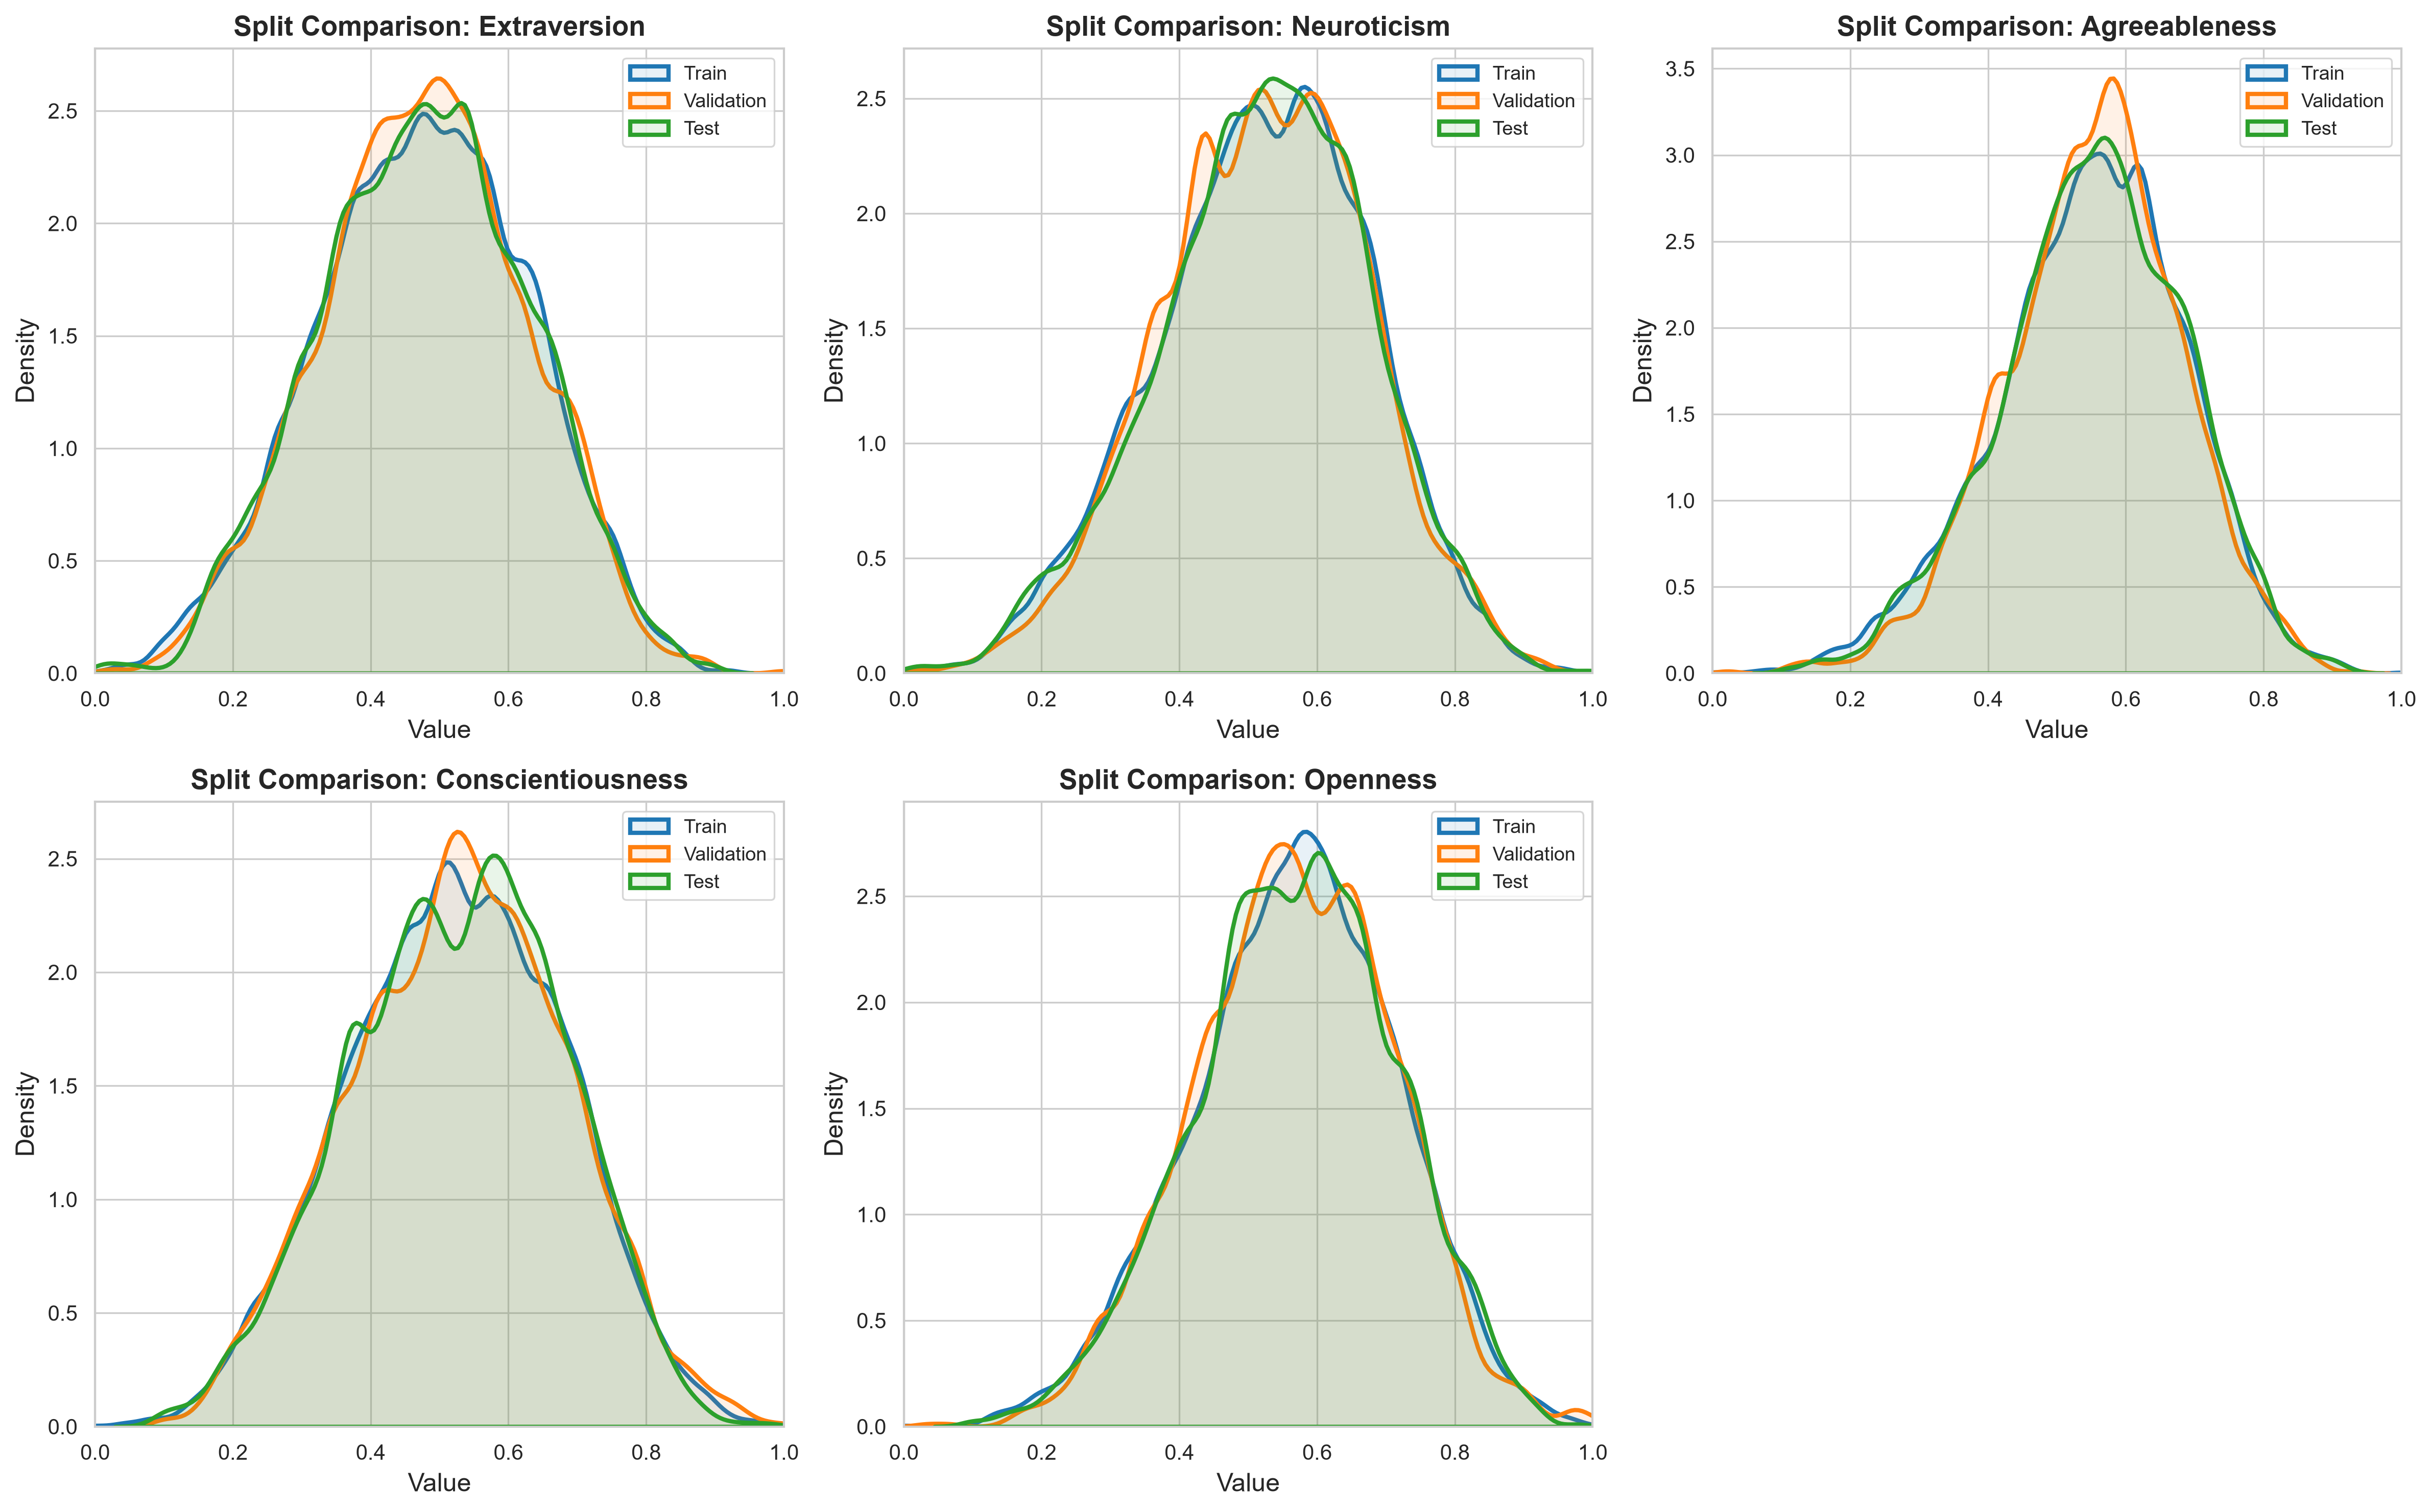
\includegraphics[width=\linewidth]{gambar/split-comparison.png}
	\caption{Perbandingan Nilai \textit{traits} pada \textit{Split} Dataset (\textit{Train, Validation, Test})}
	\label{fig:split-dataset-comparison}
\end{figure}

Berdasarkan rincian statistik yang ditunjukkan oleh \autoref{tab:statistik-dataset}, \textit{data splitting} yang dilakukan menunjukkan distribusi yang seimbang dan merata yang dibuktikan dari nilai rata-rata (\textit{mean}), standar deviasi, dan median kelima \textit{Big Five traits} yang konsisten antara data \textit{train}, \textit{validation}, dan \textit{test}. Keseragaman distribusi ini juga ditunjukkan oleh kurva densitas (\textit{density plot}) pada \autoref{fig:split-dataset-comparison} dengan perbandingan \textit{split} yang \textit{overlapping}. Sebaran label yang seimbang antar \textit{split} ini menciptakan kondisi ideal dalam pemodelan \textit{machine learning} untuk mencegah bias sekaligus menjamin bahwa evaluasi akhir pada data uji merepresentasikan kemampuan generalisasi model secara valid dan akurat.   

\begin{figure}[H]
	\centering
	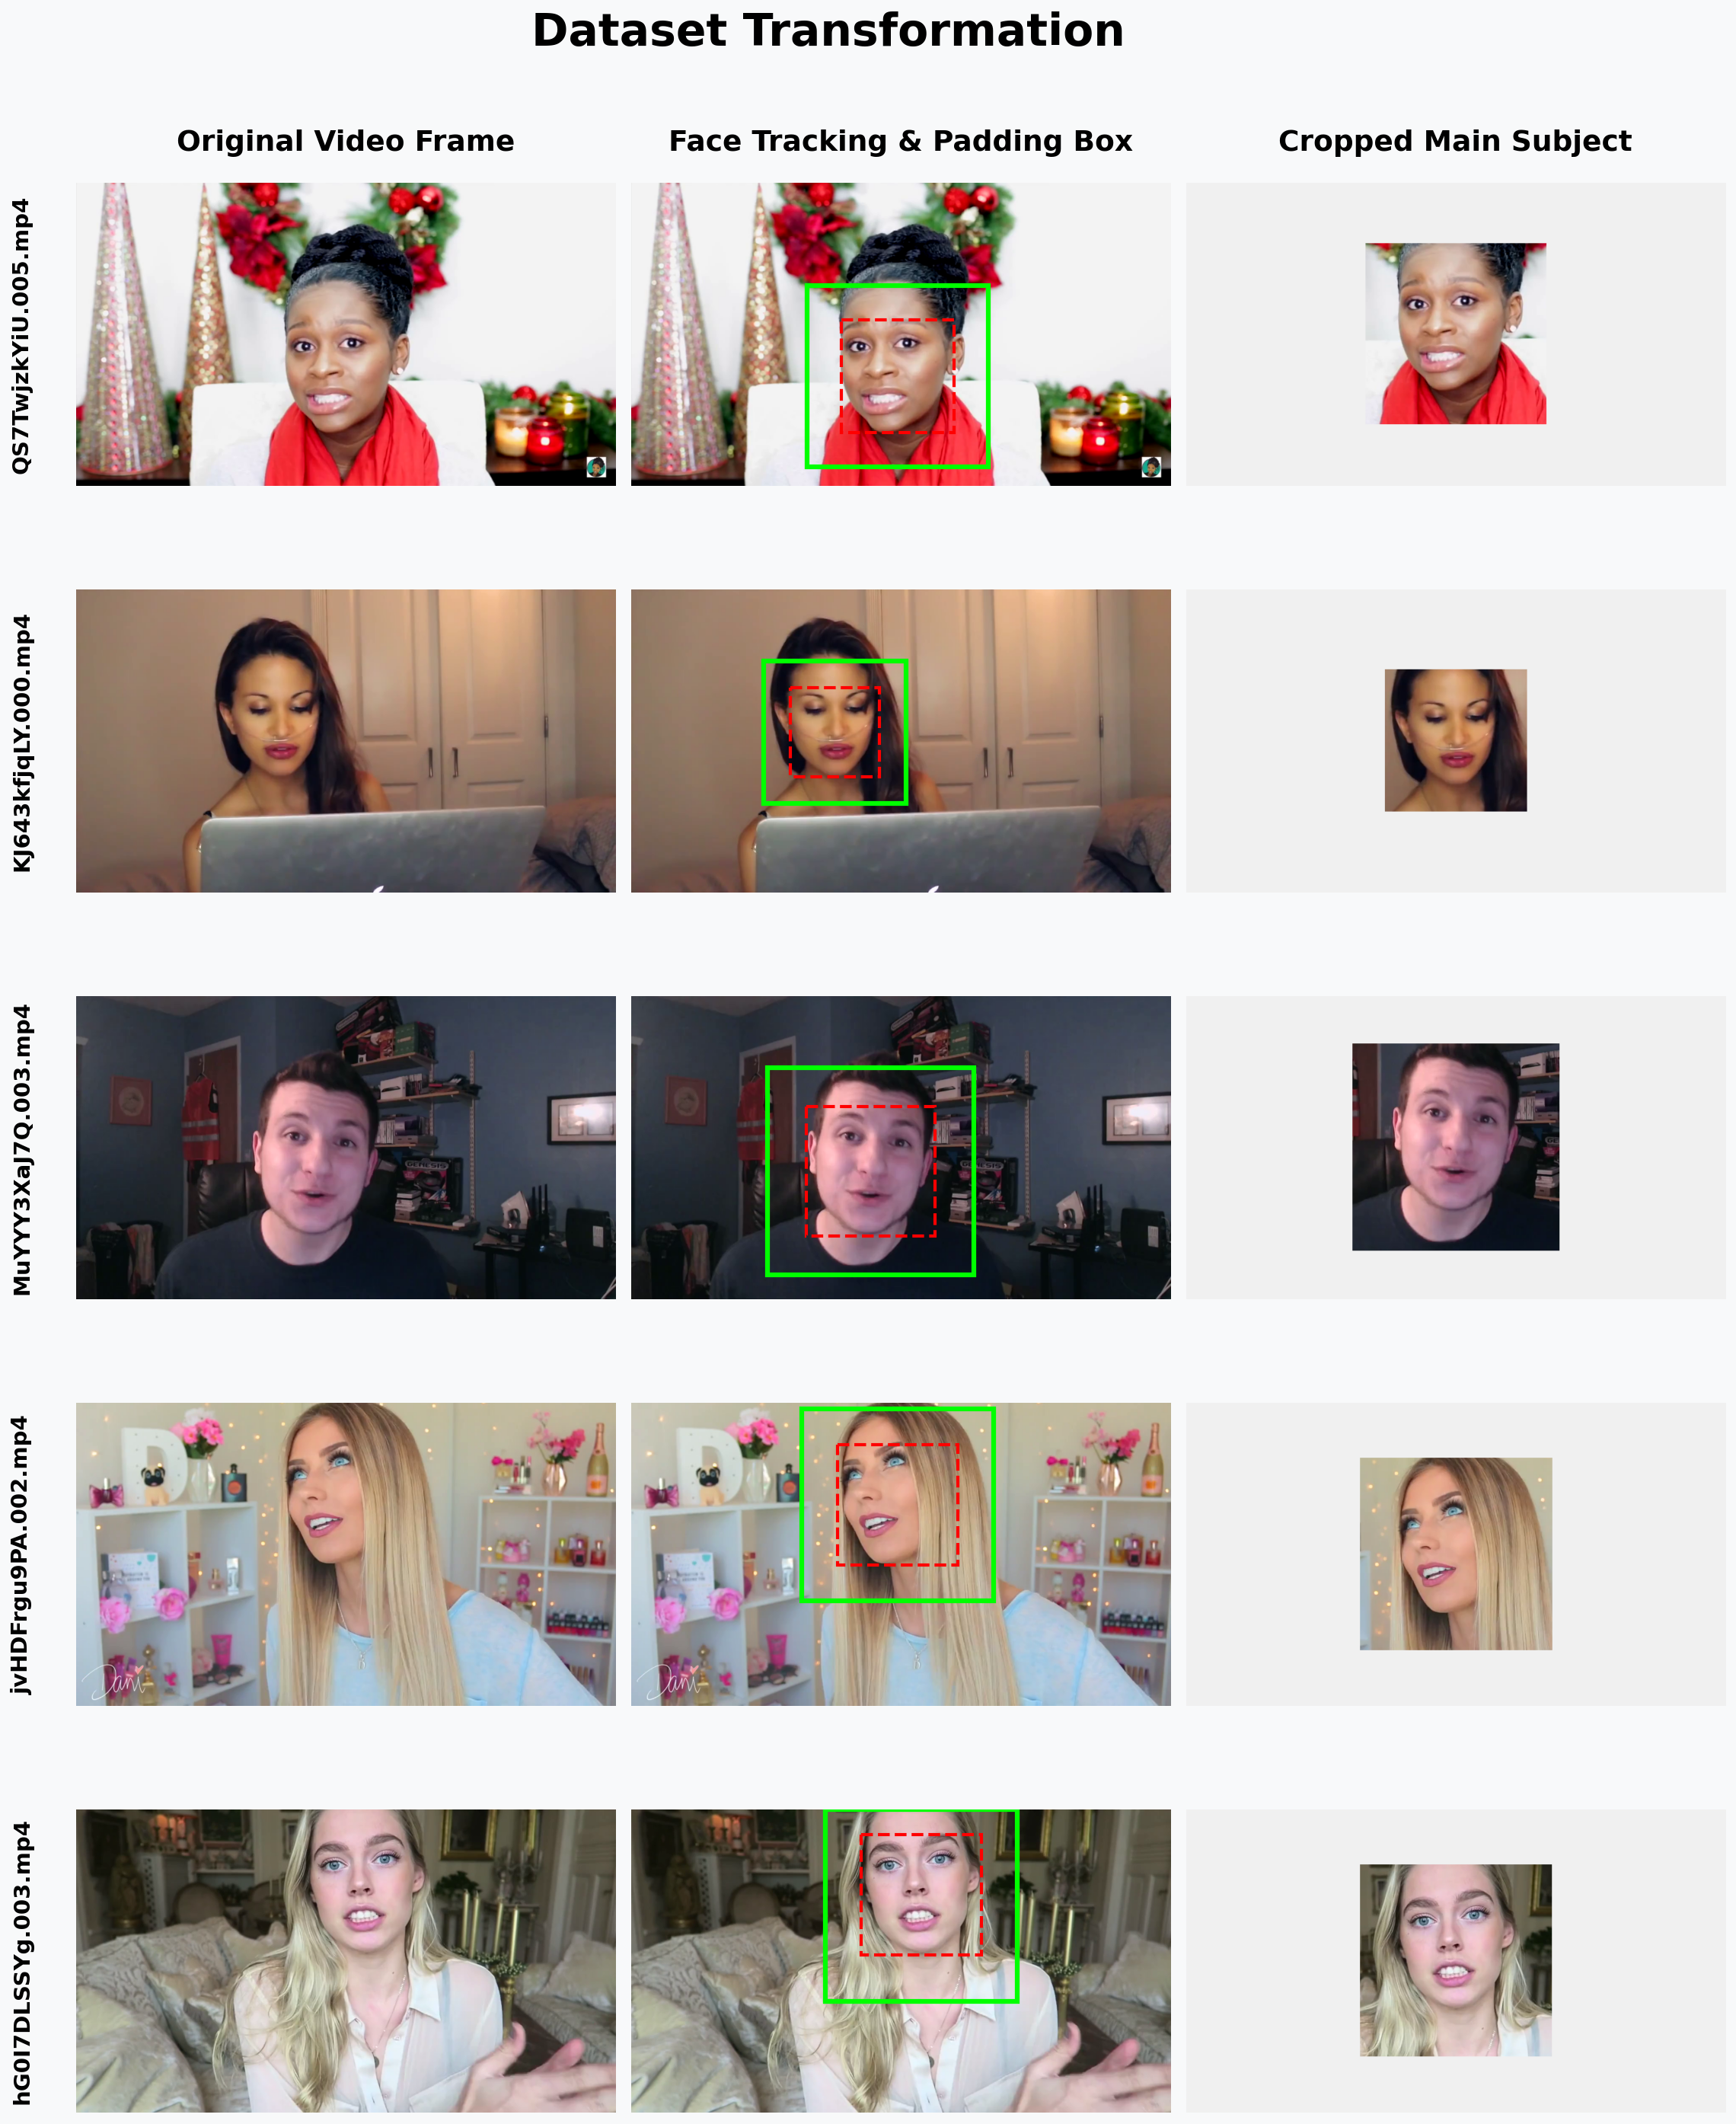
\includegraphics[width=0.83\linewidth]{gambar/dataset-transformation-steps.png}
	\caption{Proses Transformasi Dataset Video Menjadi Gambar}
	\label{fig:dataset-transform}
\end{figure}

Tahapan transformasi dataset menjadi gambar ditunjukkan oleh \autoref{fig:dataset-transform}. Setiap video dilakukan ekstraksi \textit{frame} untuk setiap satu detik durasi video sehingga rata-rata \textit{frame} yang didapatkan untuk satu video sebanyak 15 \textit{frame}. Selanjutnya untuk setiap \textit{frame} dilakukan deteksi wajah utama dan pemberian \textit{padding} sebesar 30\% agar fitur wajah seperti rambut tidak terpotong. Terakhir, dilakukan \textit{cropping} pada bagian wajah dengan \textit{padding} untuk menghapus detail latar belakang yang tidak perlu yang dapat mengganggu konvergensi model saat proses pelatihan. Hasil gambar setelah dilakukan \textit{cropping} ini yang menjadi hasil akhir transformasi dataset sebelum dilakukan praproses.
	
\subsection{Hasil Praproses Dataset}

Tahap praproses dataset dilakukan pada gambar wajah yang telah berhasil diekstraksi dan dipotong untuk memastikan kompatibilitas format input dengan arsitektur model Transformer sekaligus meningkatkan variabilitas data latih. Gambar wajah yang menjadi input awal merupakan hasil pemotongan yang membuang latar belakang tidak relevan dengan tetap mempertahankan fitur identitas utama subjek seperti yang terlihat pada variasi sampel gambar dengan skor kepribadian \textit{Big Five} yang ditunjukkan \autoref{fig:dataset-sample-bigfive}.

\begin{figure}[H]
	\centering
	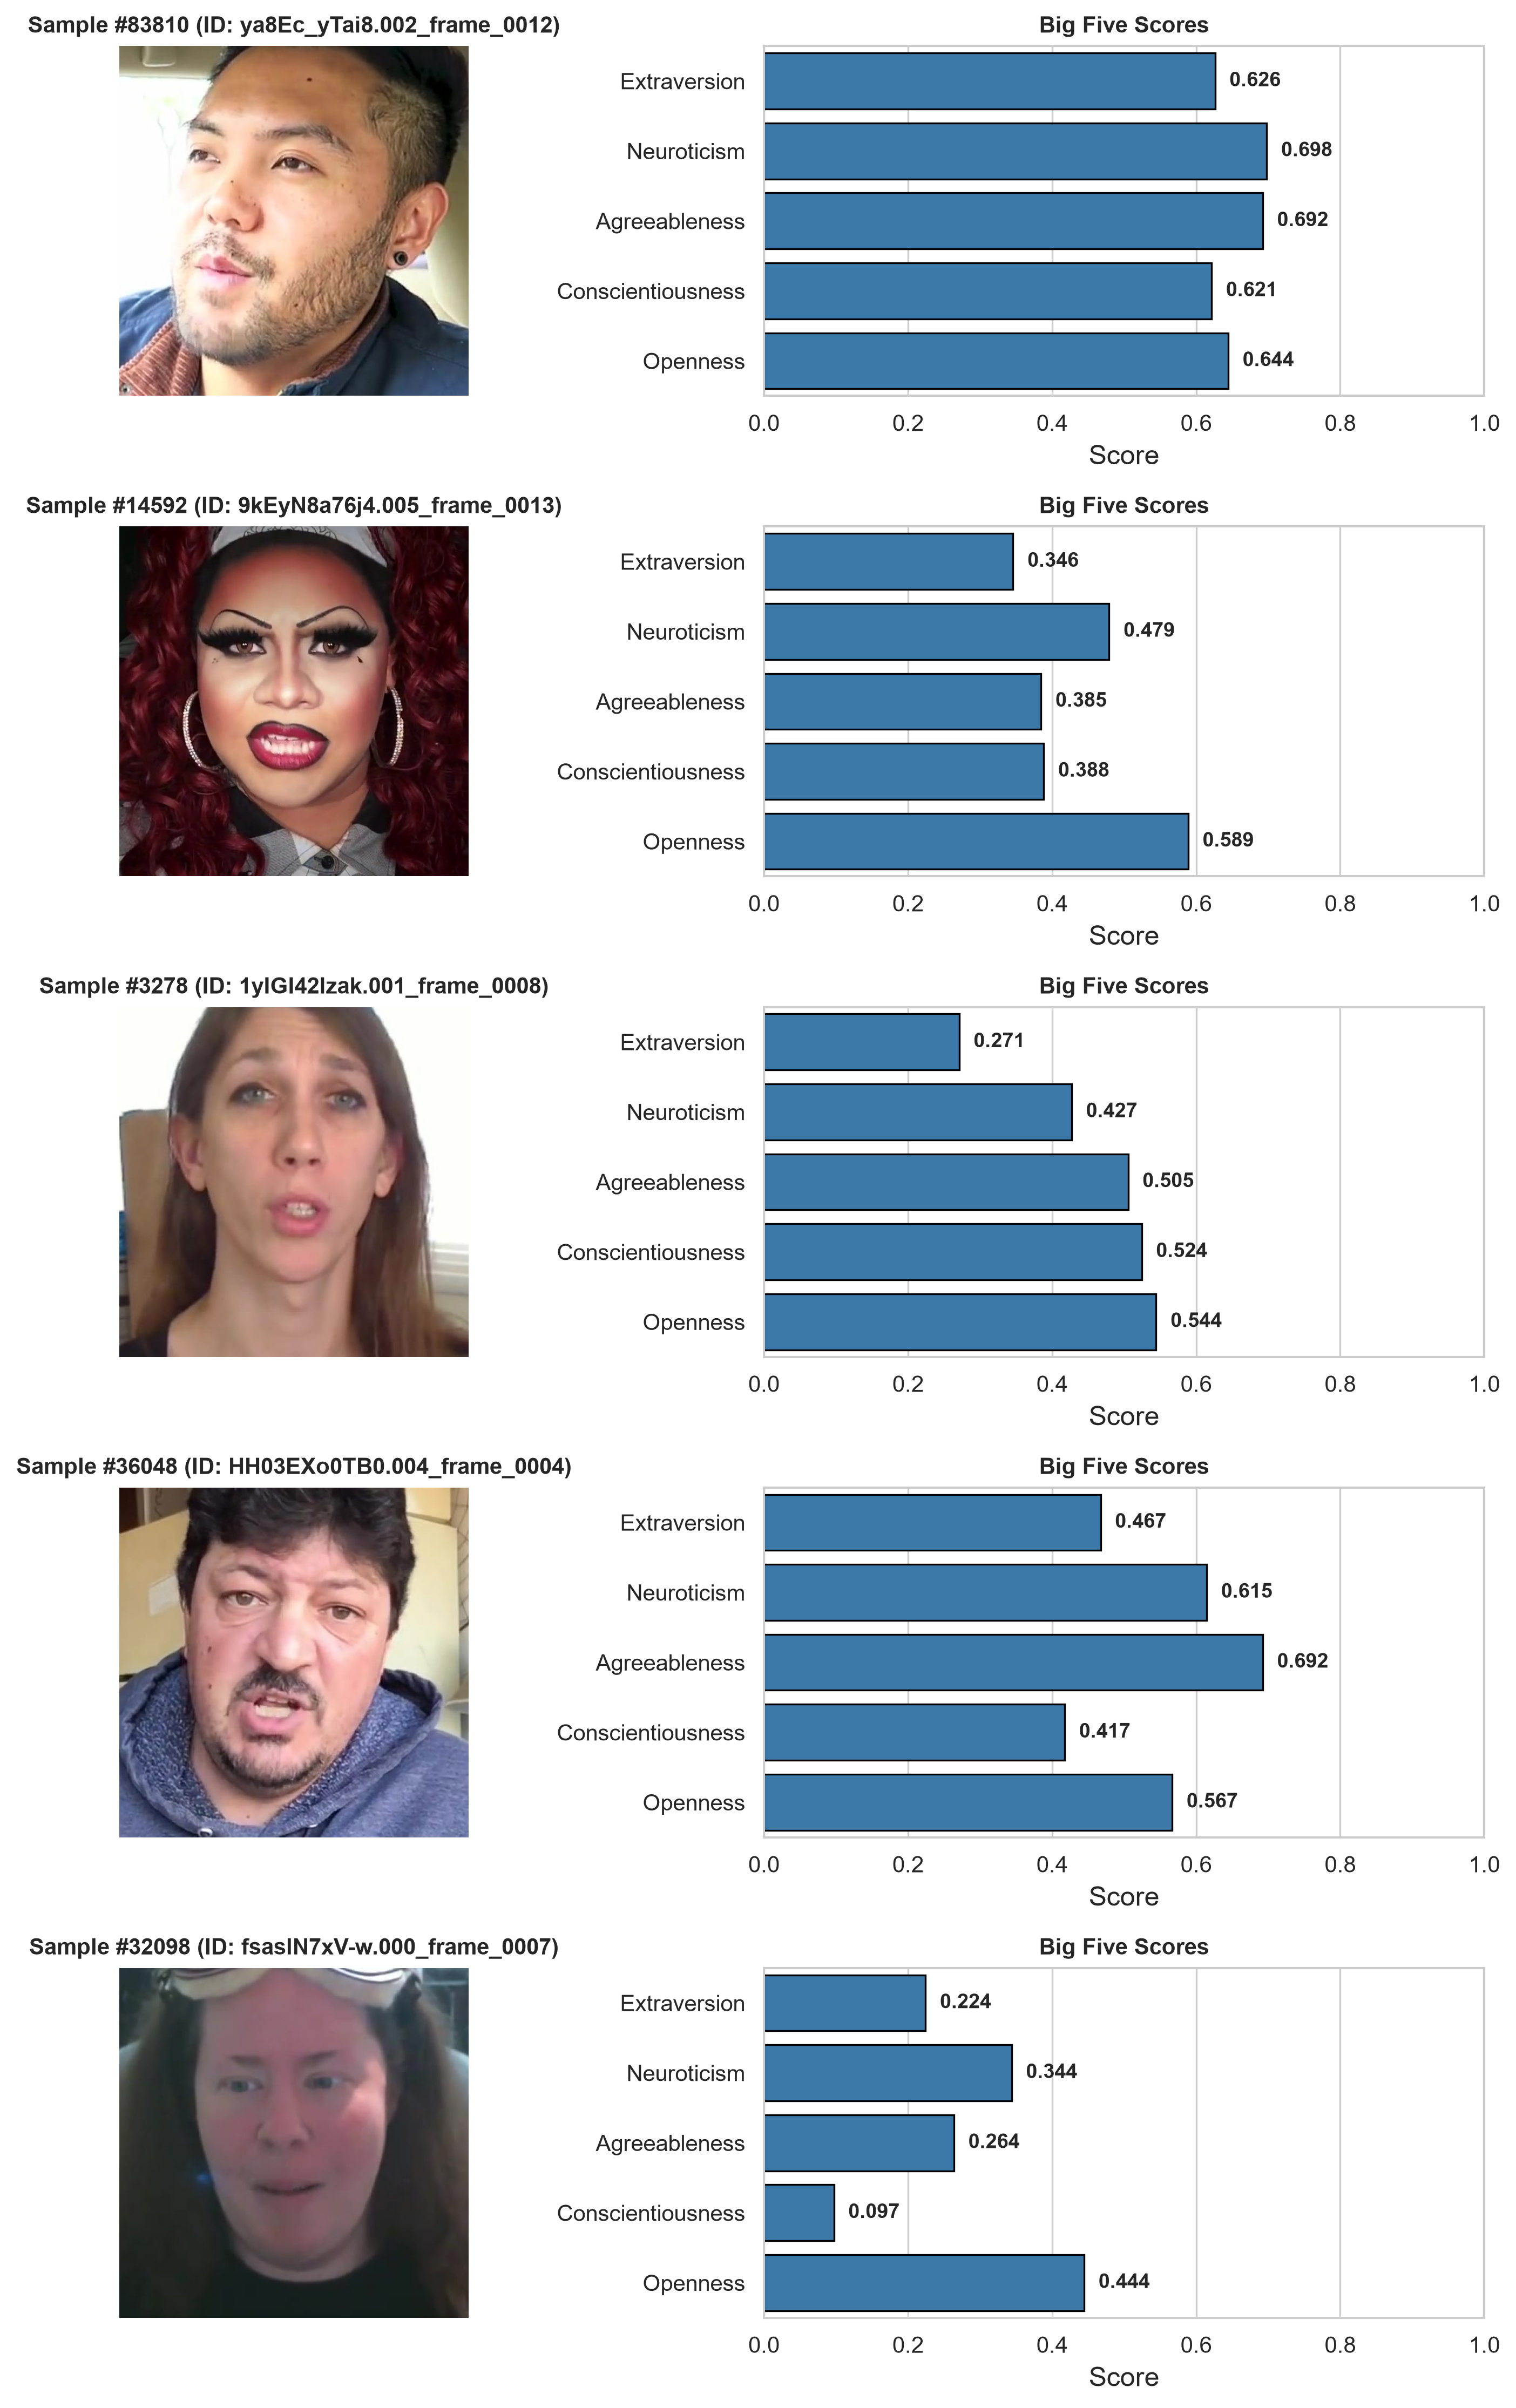
\includegraphics[width=0.75\linewidth]{gambar/sample-images-with-traits.png}
	\caption{Contoh Sampel Gambar pada Dataset dengan Skor Kepribadian \textit{Big Five}}
	\label{fig:dataset-sample-bigfive}
\end{figure}

Berdasarkan \autoref{fig:augmentation-transformation}, alur praproses ini diawali dengan pengubahan ukuran gambar (\textit{resizing}) menjadi resolusi seragam, yakni $224\times224$ piksel untuk standar input model ViT dan PVTv2, serta $256\times256$ piksel untuk model Swin Transformer V2. Setelah itu, guna mencegah terjadinya \textit{overfitting} serta memperkaya representasi fitur visual yang akan dipelajari oleh model, gambar melewati serangkaian proses augmentasi data. Tahapan augmentasi ini secara berurutan meliputi \textit{horizontal flip} dengan probabilitas acak sebesar 0,5, \textit{rotation} secara acak dalam rentang $\pm 10^{\circ}$, dan modifikasi tingkat kecerahan serta kontras (\textit{color jitter}) dengan faktor maksimal 0,2. Rangkaian praproses ini kemudian diakhiri dengan tahap mengonversi matriks piksel gambar menjadi representasi tensor yang dilanjutkan dengan penerapan normalisasi. Proses normalisasi tersebut menyesuaikan nilai distribusi warna pada gambar menggunakan parameter \textit{Z-score} sehingga seluruh data gambar terstandarisasi secara optimal dan siap untuk diproses oleh lapisan \textit{backbone} pada model prediksi.

\begin{figure}[H]
	\centering
	\includegraphics[width=\linewidth]{gambar/transformations-augmentation-visualization.png}
	\caption{Tahap Praproses Gambar dengan Augmentasi}
	\label{fig:augmentation-transformation}
\end{figure}

\subsection{Hasil Pelatihan Model Prediksi Kepribadian}

Bagian ini menyajikan pemaparan mengenai hasil pelatihan model regresi untuk prediksi kepribadian \textit{Big Five} berdasarkan ekstraksi fitur visual wajah. Pelatihan model menggunakan enam varian model \textit{pretrained} berbasis Transformer yang mencakup variasi dari ViT, Swin Transformer V2, dan PVTv2. Untuk mengidentifikasi pengaruh modifikasi arsitektur dan variabilitas data terhadap kinerja pelatihan, pengujian dilakukan melalui empat skenario eksperimen yang berbeda, yakni \textit{baseline}, \textit{arch tuning}, augmentasi, dan kombinasi \textit{arch tuning} beserta augmentasi. Melalui pendekatan komparatif pada berbagai skenario ini, analisis ditujukan untuk mengevaluasi sejauh mana integrasi antara teknik augmentasi gambar dan penyesuaian struktur \textit{regression head} memengaruhi stabilitas konvergensi metrik \textit{loss} (MAE) selama fase \textit{training} dan \textit{validation} sekaligus menentukan konfigurasi paling optimal dalam menghasilkan nilai prediksi akhir pada setiap model.

\begin{figure}[H]
	\centering
	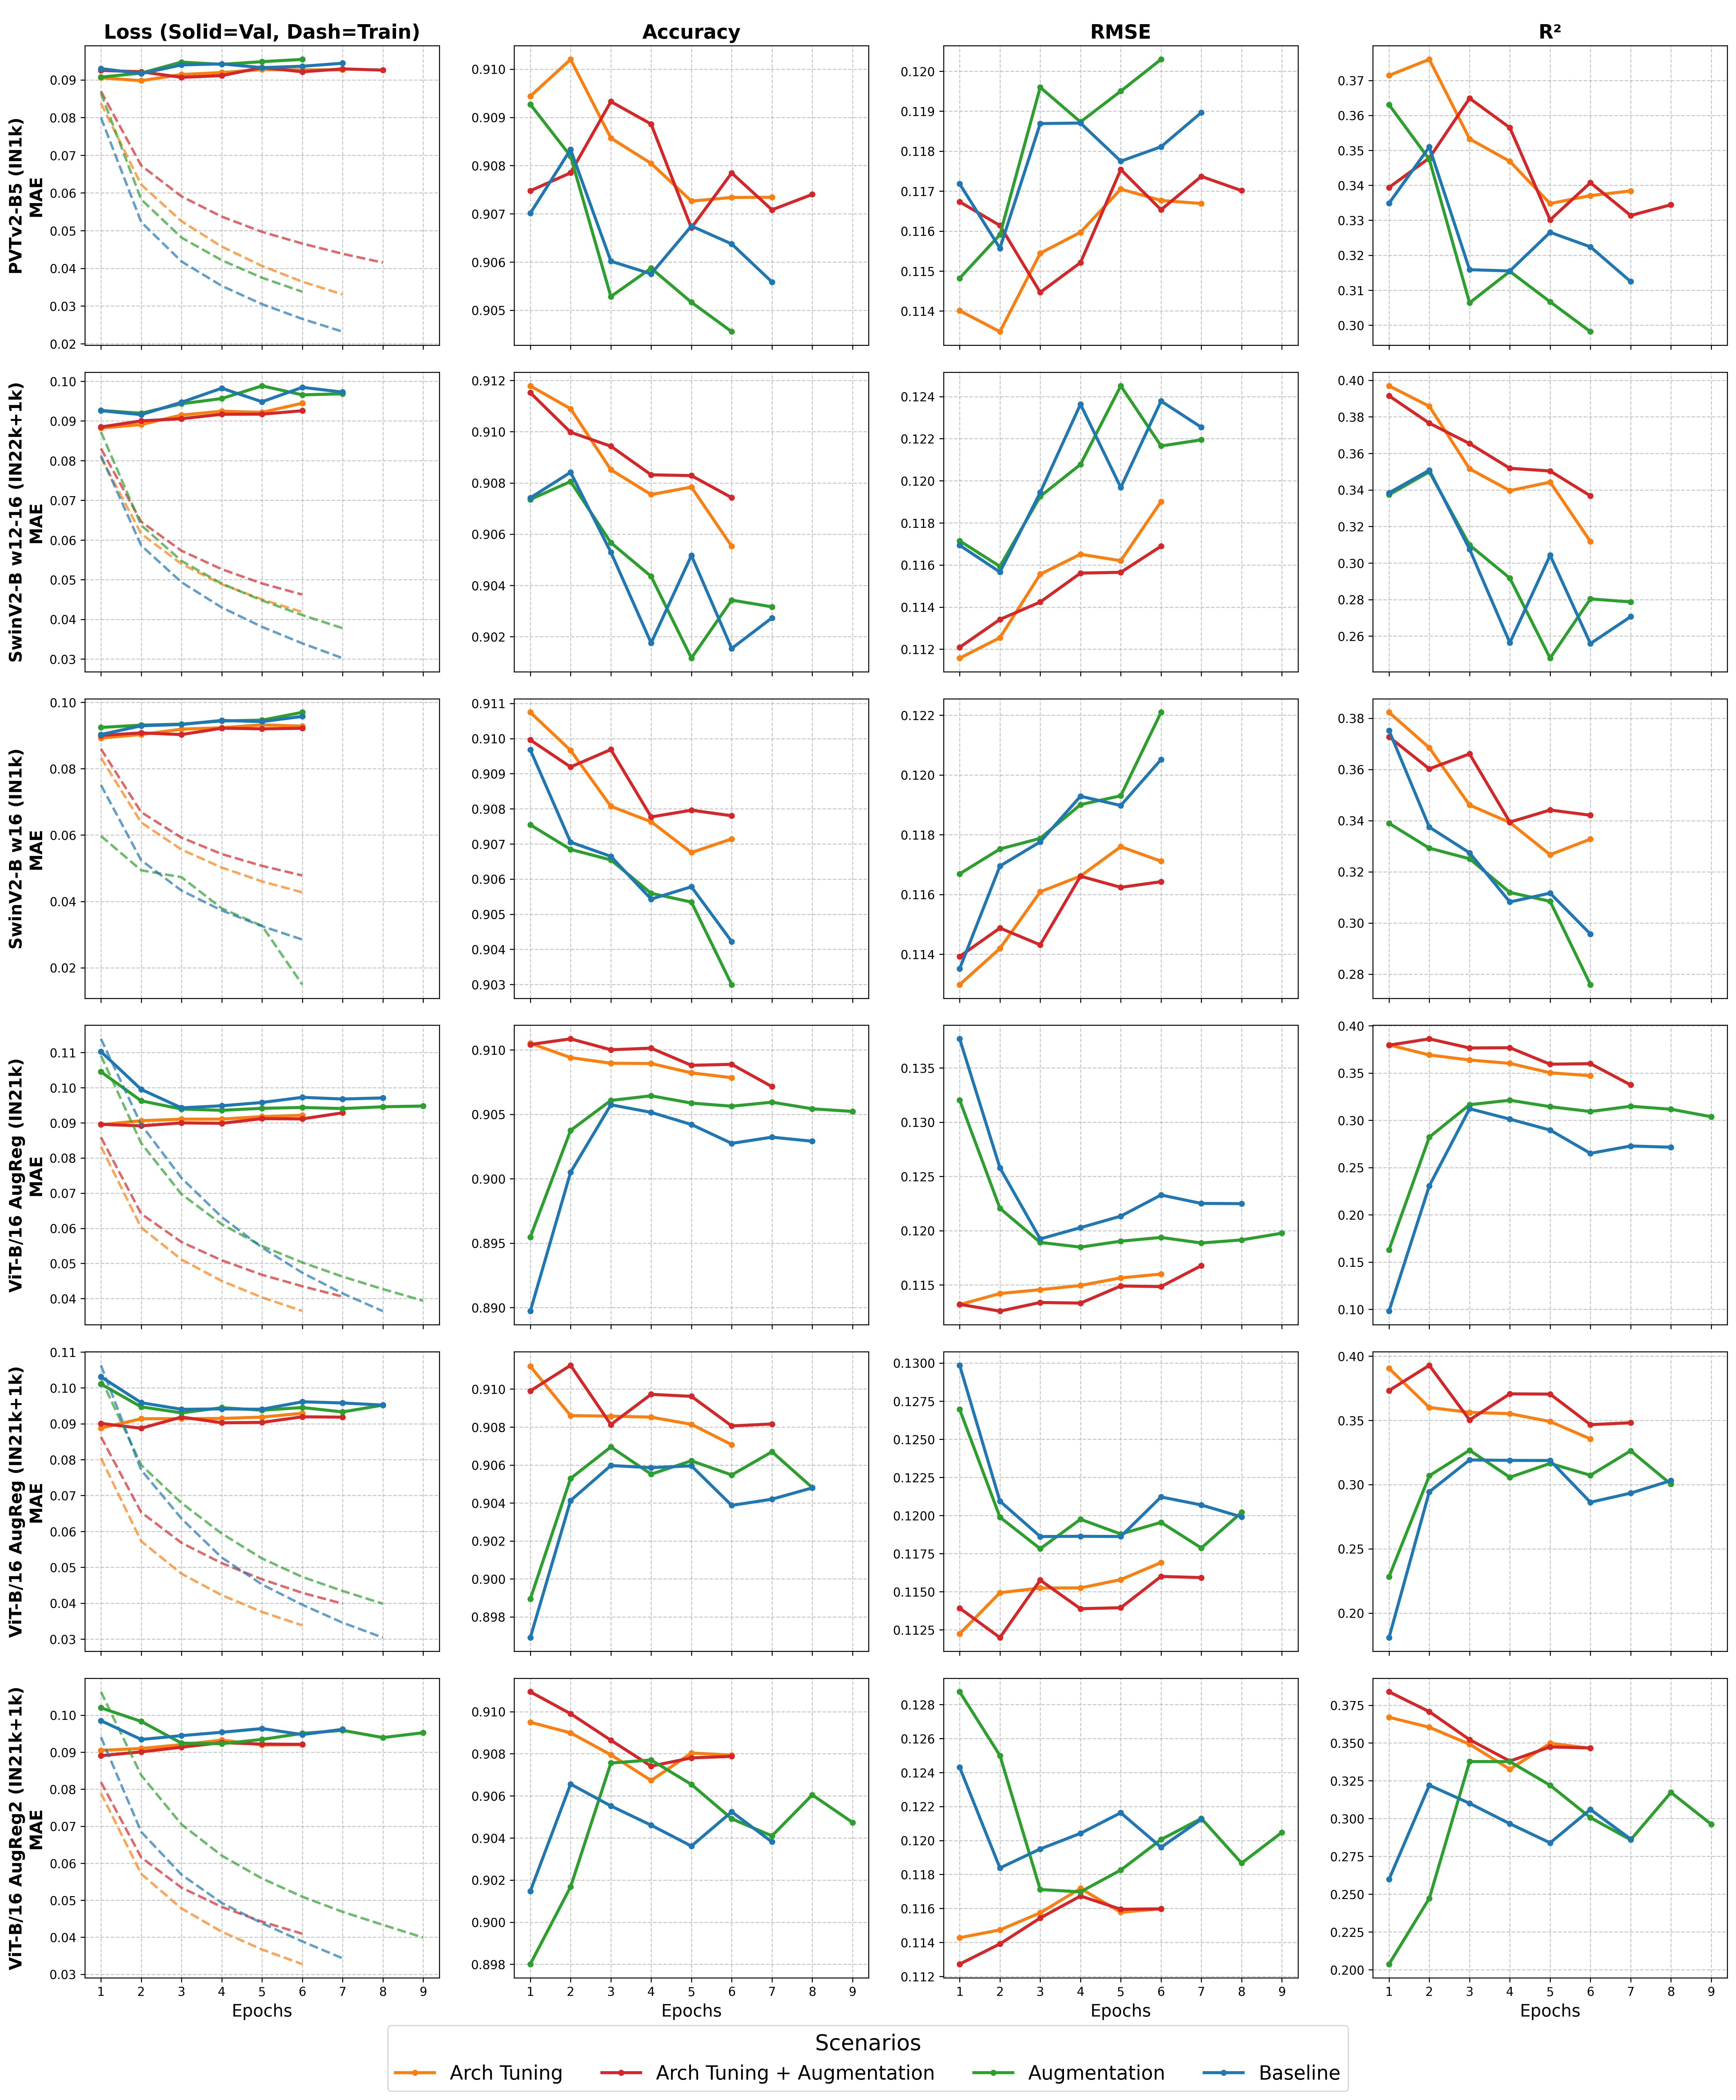
\includegraphics[width=\linewidth]{gambar/all-models-learning-dynamics.png}
	\caption{Grafik Pelatihan Setiap Model pada Setiap Skenario}
	\label{fig:train-learning-dynamics}
\end{figure}

Berdasarkan visualisasi dinamika pembelajaran yang ditunjukkan pada \autoref{fig:train-learning-dynamics}, model menunjukkan pola konvergensi yang bervariasi selama fase pelatihan dan validasi. Pada kolom metrik \textit{Loss} (MAE), terlihat bahwa seluruh model berhasil mempelajari pola dari data latih yang ditandai dengan penurunan kurva \textit{training loss} secara konsisten di setiap \textit{epoch}. Namun, nilai \textit{validation loss} cenderung stagnan setelah beberapa \textit{epoch} awal. Kondisi ini memicu mekanisme \textit{early stopping} yang umumnya terjadi antara \textit{epoch} 6 hingga 9 untuk menghentikan proses pelatihan lebih awal guna mencegah terjadinya \textit{overfitting} di mana model terlalu mengingat data latih namun gagal menggeneralisasi data baru. Hal ini menunjukkan model \textit{pretrained} berbasis Transformer cenderung mengalami konvergensi yang cepat pada data validasi yang terjadi pada \textit{epoch} 1 atau 2.

Ditinjau dari pengaruh skenario pengujian, implementasi \textit{custom regression head} memiliki dampak yang cukup signifikan. Skenario \textit{arch tuning} dan \textit{arch tuning + augmentation} secara konsisten mendominasi metrik kinerja di hampir seluruh arsitektur \textit{backbone}. Kedua skenario ini mendapatkan nilai \textit{accuracy} dan \textit{Coefficient of Determination} ($R^2$) yang lebih tinggi, serta nilai \textit{error} (RMSE dan MAE) yang lebih rendah dibandingkan dengan skenario \textit{baseline}. Di sisi lain, penerapan augmentasi gambar tanpa penyesuaian arsitektur menunjukkan kinerja paling tidak stabil dan sering kali berada di bawah kinerja \textit{baseline}, khususnya pada arsitektur ViT-B/16. Hal ini menunjukkan bahwa variabilitas data visual yang dihasilkan dari proses augmentasi memerlukan kapasitas representasi yang lebih kompleks dari \textit{custom regression head} agar dapat dipetakan secara optimal menjadi prediksi skor kepribadian yang akurat. Secara umum, penerapan augmentasi dan penggunaan
\textit{custom regression head} yang lebih kompleks berdampak pada peningkatan kinerja pelatihan model yang lebih baik dengan mengurangi risiko \textit{overfitting} dini, sekaligus memperkuat kemampuan generalisasi model saat dihadapkan pada variasi data visual yang belum pernah dilihat sebelumnya. 

\begin{figure}[H]
	\centering
	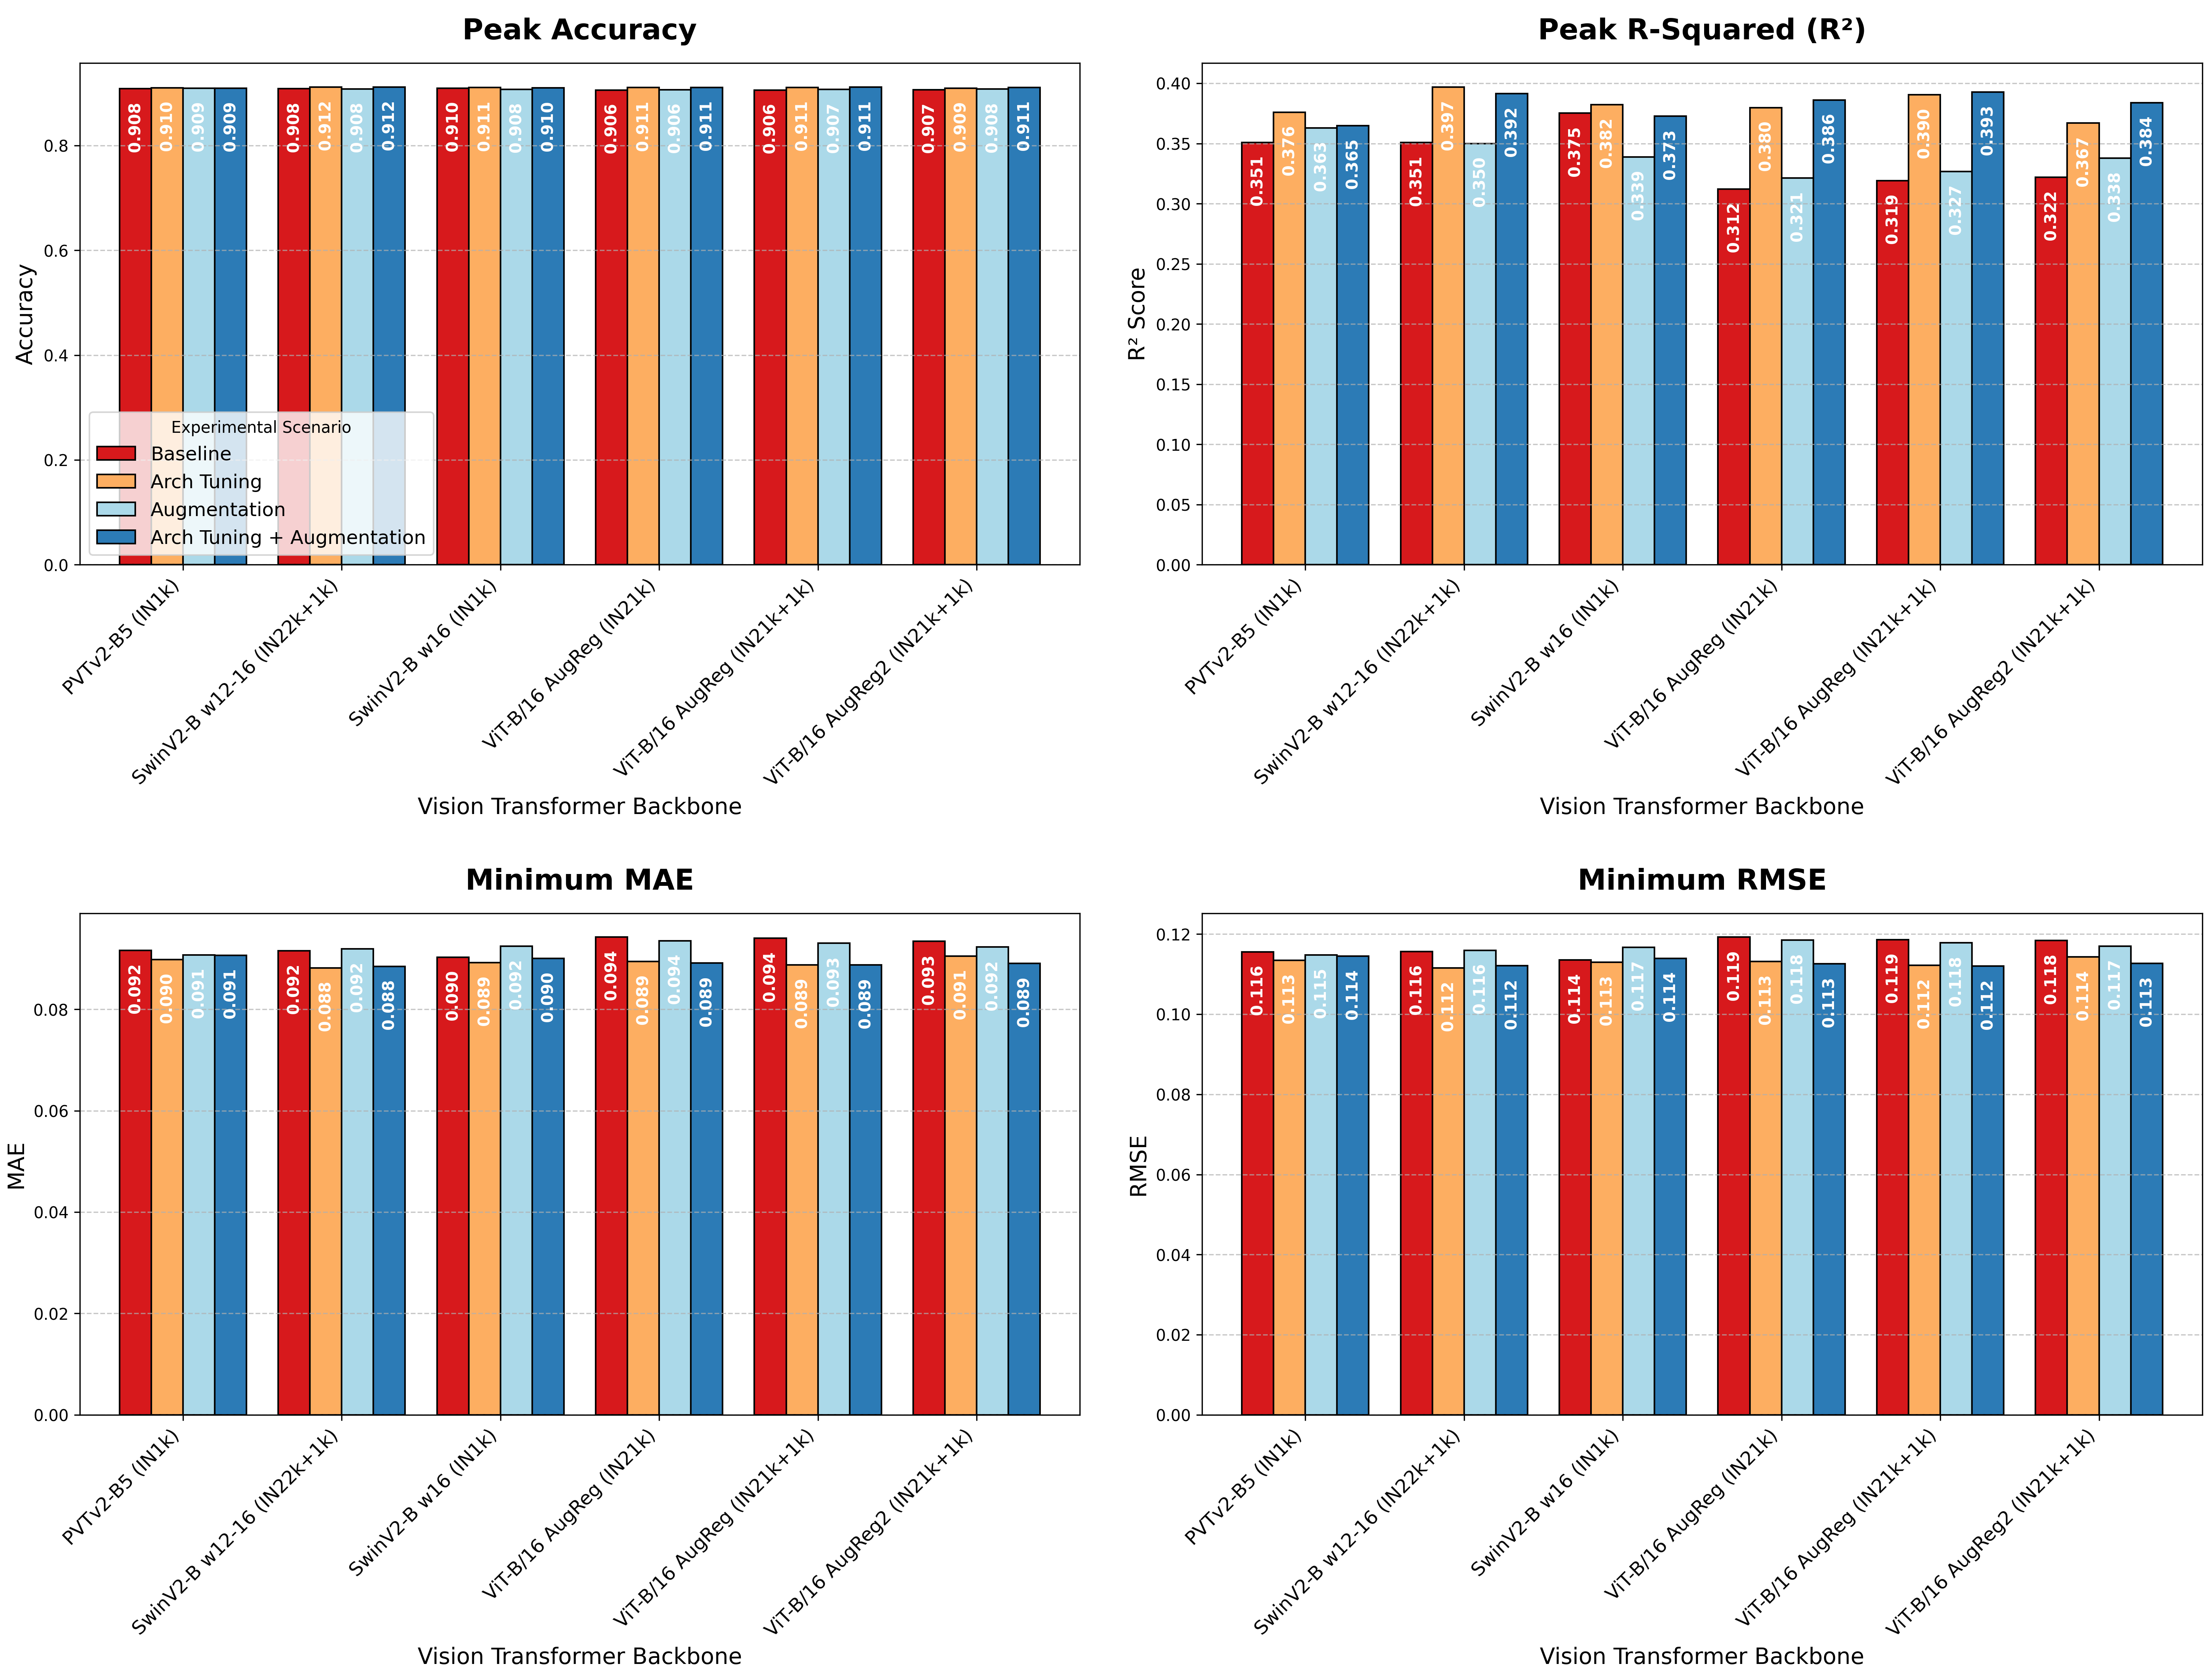
\includegraphics[width=0.9\linewidth]{gambar/bar-all-val-metrics.png}
	\caption{Metrik Kinerja Terbaik Model pada Proses Pelatihan}
	\label{fig:best-metrics-training}
\end{figure}

Berdasarkan grafik perbandingan kinerja terbaik pada \autoref{fig:best-metrics-training}, terdapat pola yang konsisten mengenai dampak dari penerapan skenario terhadap kinerja keseluruhan model. Secara umum, skenario yang mengimplementasikan \textit{custom regression head} kompleks, yaitu \textit{arch tuning} dan kombinasi \textit{arch tuning + augmentation} mengungguli skenario \textit{baseline} pada seluruh varian model. Keunggulan ini ditandai dengan pencapaian nilai \textit{peak accuracy} dan \textit{peak R-squared} ($R^2$) yang lebih tinggi sekaligus tingkat \textit{error} (Minimum MAE dan Minimum RMSE) yang lebih rendah. Jika dilihat dari perbandingan kinerja terbaik antara model-model yang dilatih, tidak terdapat perbedaan yang signifikan pada tingkat \textit{error} (MAE dan RMSE) maupun \textit{accuracy}. Akan tetapi, perbedaan penerapan skenario terhadap kinerja model menjadi sangat jelas ditinjau dari metrik \textit{coefficient of determination} ($R^2$). Metrik ini menjelaskan kemampuan model dalam menjelaskan varians atau pola persebaran data skor kepribadian yang tidak hanya meminimalkan rata-rata selisih kesalahan. Berdasarkan grafik \textit{Peak R-Squared}, dapat dilihat bahwa implementasi \textit{custom regression head} (pada skenario \textit{arch tuning} dan \textit{arch tuning + augmentation}) memicu kenaikan nilai $R^2$ yang signifikan secara konsisten pada seluruh model jika dibandingkan dengan kinerja \textit{baseline}. Peningkatan secara umum ini menunjukkan bahwa arsitektur \textit{head} standar (\textit{baseline}) yang berupa lapisan linier sederhana tidak memiliki kapasitas representasi yang cukup untuk memetakan fitur visual ke dalam ruang regresi kontinu \textit{multi target}. Penambahan kompleksitas pada \textit{custom regression head} melalui penambahan dimensi lapisan \textit{fully connected}, penerapan fungsi aktivasi \textit{non linear} GELU, serta regularisasi \textit{dropout} memberikan kapabilitas matematis yang dibutuhkan oleh model. Komponen ini meningkatkan kapasitas model dalam menangkap keunikan profil kepribadian setiap individu secara spesifik sehingga model dapat menghindari kecenderungan untuk selalu memprediksi nilai rata-rata secara konstan.

Analisis spesifik terhadap kinerja (\textit{peak metrics}) pada fase validasi menunjukkan bahwa model SwinV2-B w12-16 (IN22k+1k) memberikan kinerja terbaik selama proses pelatihan berlangsung. Pada skenario \textit{arch tuning}, model ini berhasil mencapai rekor kinerja validasi tertinggi dengan nilai \textit{peak accuracy} mencapai 0,912 dan \textit{Coefficient of Determination} ($R^2$) sebesar 0,397. Keunggulan tersebut sejalan dengan kemampuannya meminimalkan tingkat kesalahan prediksi pada data validasi yang ditunjukkan dari nilai \textit{MAE} terendah di angka 0,088 dan \textit{minimum RMSE} sebesar 0,112. Meskipun varian model lain seperti ViT-B/16 dan PVTv2-B5 menunjukkan hasil yang tidak berbeda jauh saat menggunakan \textit{custom regression head}, SwinV2-B w12-16 tetap menjadi model dengan kinerja terbaik secara konsisten melalui instrumen evaluasi pada tahap ini. Secara teori, keunggulan kinerja validasi ini sangat dipengaruhi oleh mekanisme \textit{shifted window based self-attention} yang mampu membangun representasi fitur visual secara hierarkis. Mekanisme tersebut memungkinkan model untuk menangkap detail wajah yang kompleks jauh lebih efisien dibandingkan dengan arsitektur konvensional. Selain itu, dengan \textit{pre-trained knowledge} yang didapatkan dari skala dataset ImageNet-22k, SwinV2-B w12-16 menunjukkan potensi awal sebagai konfigurasi model \textit{backbone} paling kuat. Adapun pembuktian akhir mengenai kemampuan generalisasi sesungguhnya dari model-model ini dievaluasi dan dibahas lebih mendalam menggunakan data uji (\textit{test dataset}) pada \autoref{sec:pembahasan}.

\subsection{Hasil Interpretasi Kepribadian}

Sistem interpretasi kepribadian diimplementasikan pada aplikasi berbasis web yang mengintegrasikan \textit{output} model prediksi regresi dengan kemampuan generatif LLM. Seperti yang divisualisasikan pada \autoref{fig:interpretation-result-ui}, aplikasi ini menerima input berupa citra wajah yang kemudian diteruskan ke model inferensi untuk mendapatkan skor probabilitas kepribadian \textit{Big Five}. Skor numerik tersebut kemudian disusun bersama dengan data citra dalam bentuk \textit{prompt} dan dikirimkan menuju layanan LLM pilihan pengguna seperti Gemma 4 atau Qwen3-VL untuk diterjemahkan menjadi sebuah narasi profil psikologis yang komprehensif. Setelah proses selesai, pengguna dapat melihat skor kepribadian \textit{Big Five} dan hasil interpretasi LLM secara langsung.

\begin{figure}[H]
	\centering
	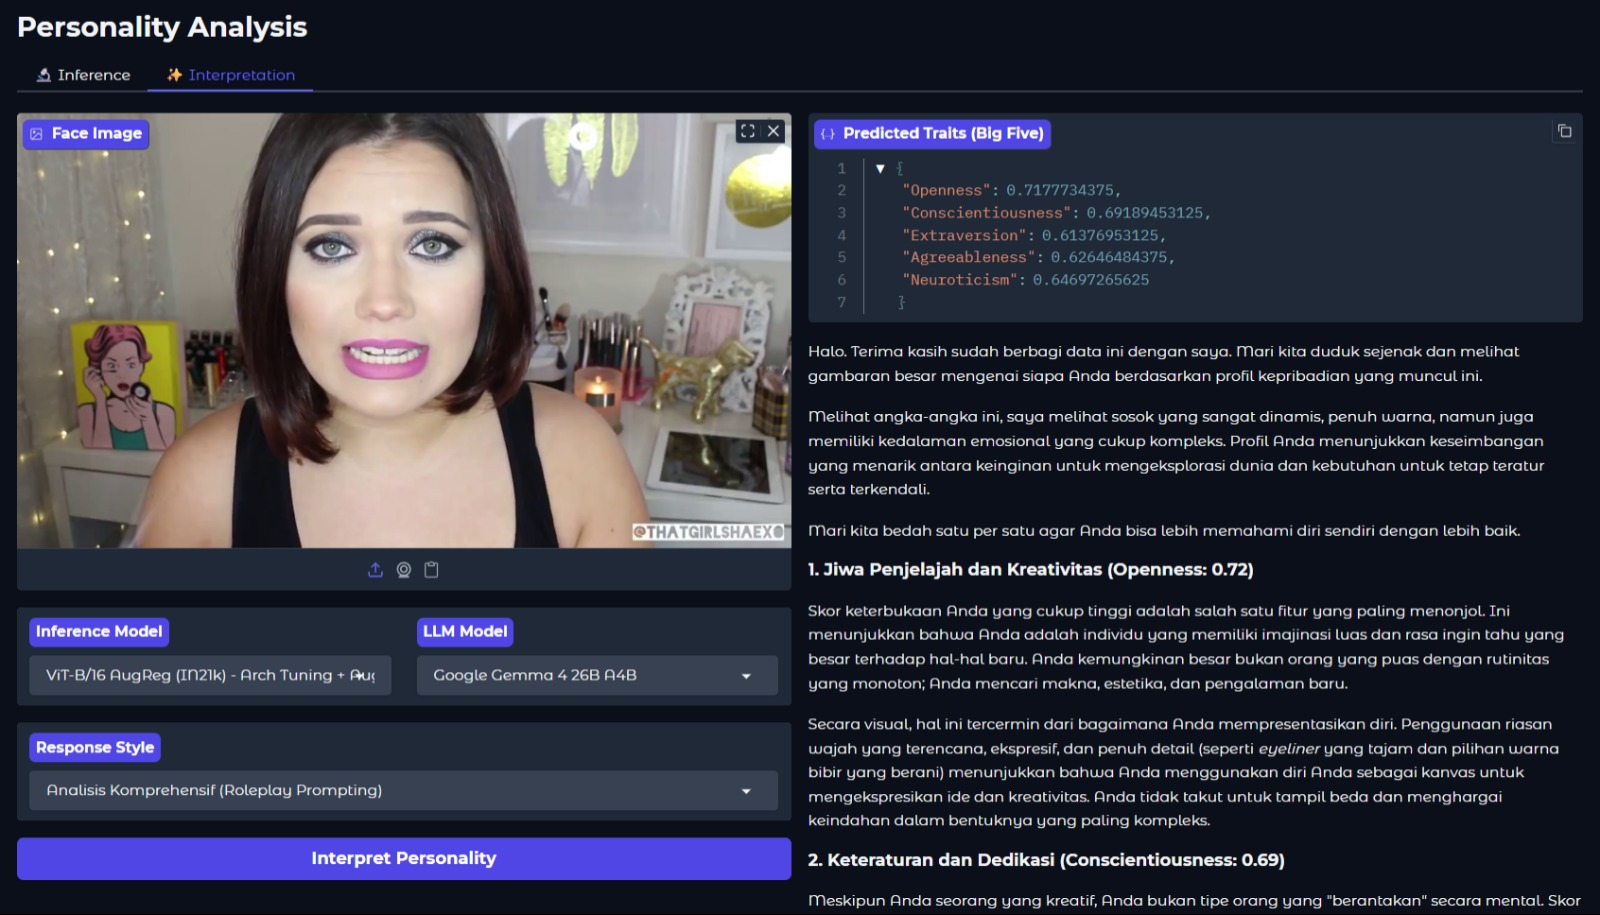
\includegraphics[width=\linewidth]{gambar/interpretation-result-example.png}
	\caption{Contoh Hasil Interpretasi Kepribadian pada Antarmuka Pengguna}
	\label{fig:interpretation-result-ui}
\end{figure}

Observasi terhadap hasil interpretasi menunjukkan adanya perbedaan karakteristik dalam cara setiap model merespons \textit{prompt} yang diberikan. Berdasarkan visualisasi perbandingan \textit{output} yang ditunjukkan pada \autoref{fig:gemma-interpretation-comparison} dan \autoref{fig:qwen-interpretation-comparison}, model Gemma 4 memiliki kecenderungan untuk menghasilkan narasi yang ringkas, padat, dan terstruktur dengan sangat rapi. Pembahasan kelima ciri kepribadian \textit{Big Five} didistribusikan secara proporsional dan disampaikan menggunakan sapaan formal "Anda". Model Qwen3-VL menunjukkan karakteristik respons yang jauh lebih ekspresif dan detail, serta menggunakan gaya bahasa yang sedikit lebih santai dengan kata ganti "Kamu". Qwen3-VL cenderung sangat memperhatikan aspek visual seperti sorot mata, postur, atau elemen penampilan yang dikaitkan dengan kedalaman emosional. Akibat dari tingkat pembahasan yang lebih detail, respons dari Qwen3-VL memakan jumlah token yang jauh lebih besar dibandingkan Gemma 4 meskipun telah diberikan instruksi \textit{prompt} untuk memberikan respons tidak lebih dari 1500 token. Pada beberapa sampel pengujian, hal ini menyebabkan \textit{output} teks Qwen3-VL menyentuh batas maksimal (\textit{hard limit}) sistem sebesar 2500 token, mengakibatkan terpotongnya hasil interpretasi kepribadian.

Selain dipengaruhi oleh pilihan LLM, kualitas dan format \textit{output} juga sangat bergantung pada strategi \textit{prompt engineering} yang diterapkan. Pada skenario \textit{standard prompting}, baik Gemma 4 maupun Qwen3-VL menghasilkan teks dengan format yang sangat analitis dan memisahkan elemen evaluasi secara eksplisit. Hal ini terlihat pada \textit{output} Gemma 4 yang membagi setiap poin kepribadian ke dalam sub bagian khusus seperti "Analisis Visual" dan "Wawasan", sehingga menghasilkan narasi yang objektif layaknya sebuah draf laporan teknis. Ketika instruksi \textit{roleplay prompting} diterapkan, kedua LLM mengadopsi persona layaknya seorang konselor psikologi. Narasi berubah menjadi lebih hangat, empatik, dan interaktif menyerupai sesi dialog langsung dengan pengguna. Melalui pendekatan \textit{roleplay} ini, model tidak lagi memisahkan poin analisis secara kaku dan mampu menyusun kesan visual wajah ke dalam penjabaran karakter psikologis yang lebih natural.

\begin{figure}[H]
	\centering
	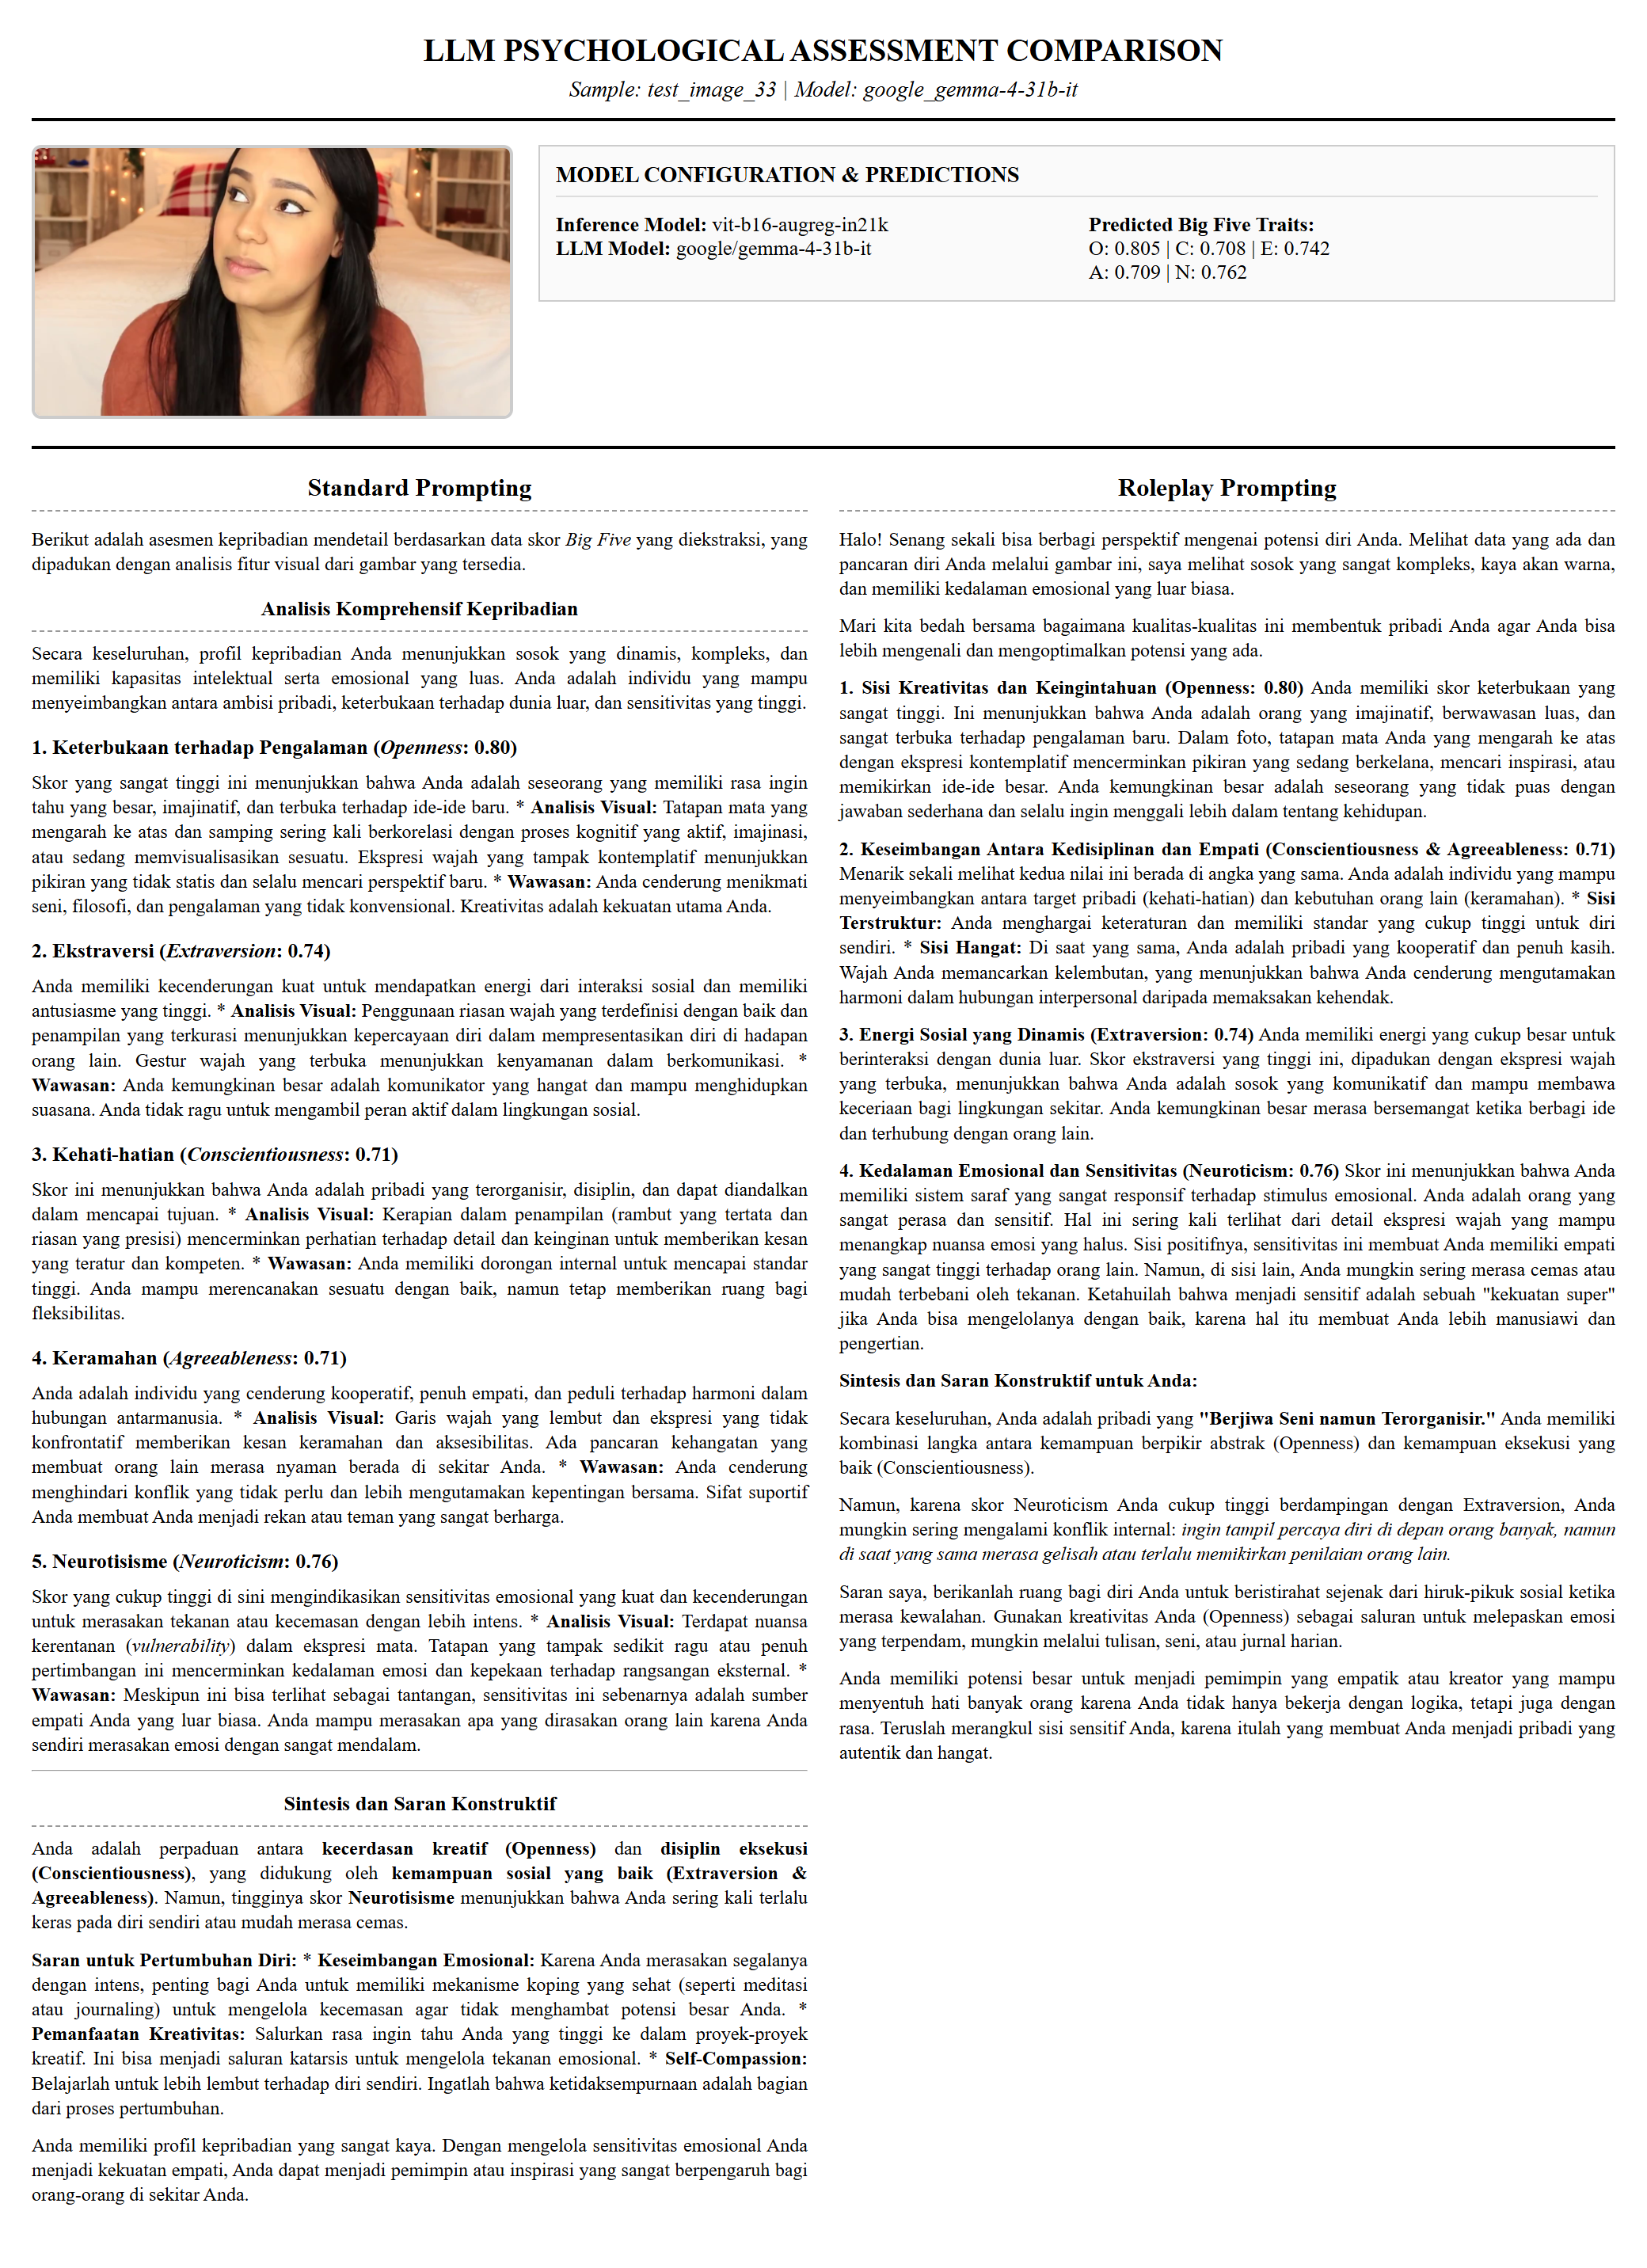
\includegraphics[width=\linewidth]{gambar/gemma-comparison-prompt.png}
	\caption{Contoh Hasil Interpretasi Kepribadian pada Model Gemma 4}
	\label{fig:gemma-interpretation-comparison}
\end{figure}

\begin{figure}[H]
	\centering
	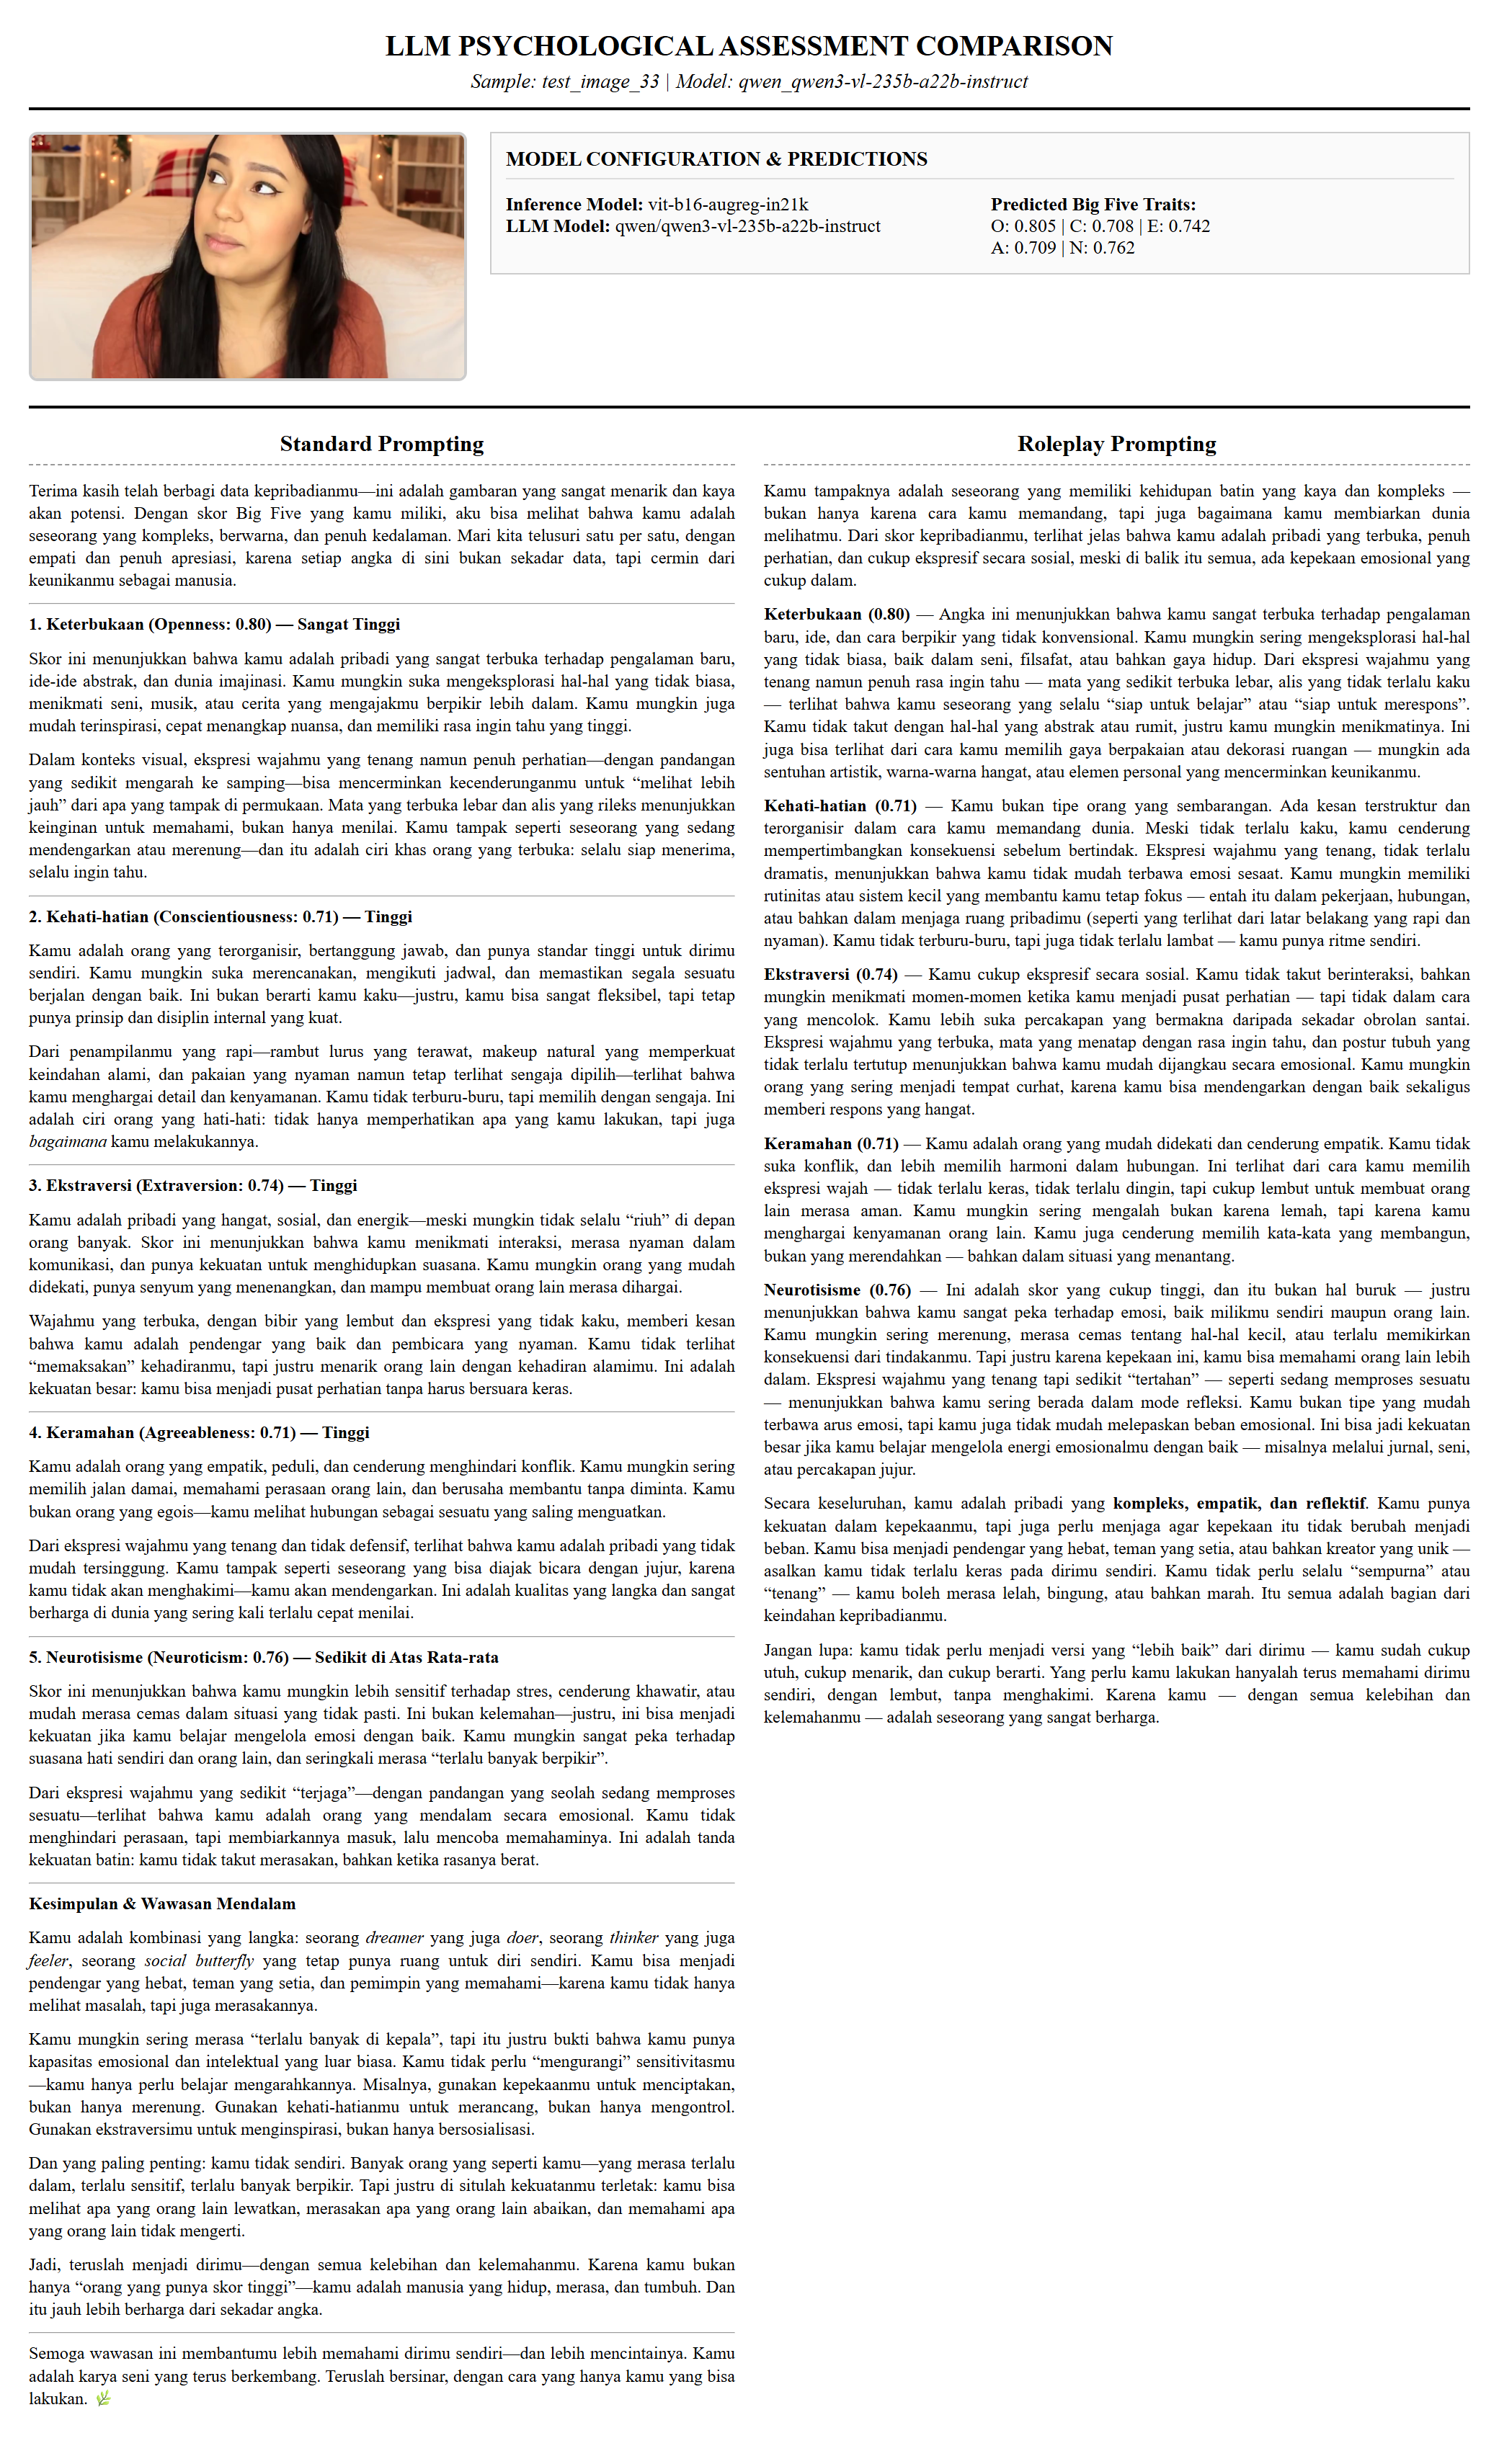
\includegraphics[width=0.9\linewidth]{gambar/qwen-comparison-prompt.png}
	\caption{Contoh Hasil Interpretasi Kepribadian pada Model Qwen3-VL}
	\label{fig:qwen-interpretation-comparison}	
\end{figure}


\section{Pembahasan}
\label{sec:pembahasan}

Bagian ini menyajikan analisis dan evaluasi terhadap sistem asesmen kepribadian hibrida yang diimplementasikan. Pembahasan diawali dengan membedah kinerja model regresi visual dalam memprediksi skor numerik kepribadian \textit{Big Five} guna menentukan arsitektur dan skenario pelatihan terbaik. Selanjutnya, fokus evaluasi dilanjutkan pada pengujian kualitas narasi interpretasi deskriptif yang dihasilkan oleh LLM berdasarkan metrik penilaian G-Eval.

\subsection{Evaluasi Model Prediksi Kepribadian}

Model prediksi yang telah dilatih melalui empat jenis skenario dievaluasi menggunakan dataset \textit{split test} untuk menentukan model dengan kinerja terbaik secara keseluruhan. Evaluasi pada data uji ini dilakukan untuk mengukur kemampuan generalisasi model secara objektif saat dihadapkan pada variasi gambar wajah yang belum pernah dilihat sebelumnya selama fase pelatihan. Berdasarkan metrik evaluasi akhir yang ditunjukkan pada \autoref{fig:test-set-metrics}, skenario yang menggunakan \textit{custom regression head} kompleks menunjukkan keunggulan dibandingkan skenario lainnya. Skenario \textit{arch tuning} dan kombinasi \textit{arch tuning + augmentation} mendominasi pencapaian tingkat kesalahan terendah pada \textit{test} MAE dan \textit{test} RMSE sekaligus menghasilkan tingkat akurasi prediksi yang lebih tinggi dibandingkan dengan skenario \textit{baseline} maupun augmentasi.   

\begin{figure}[H]
	\centering
	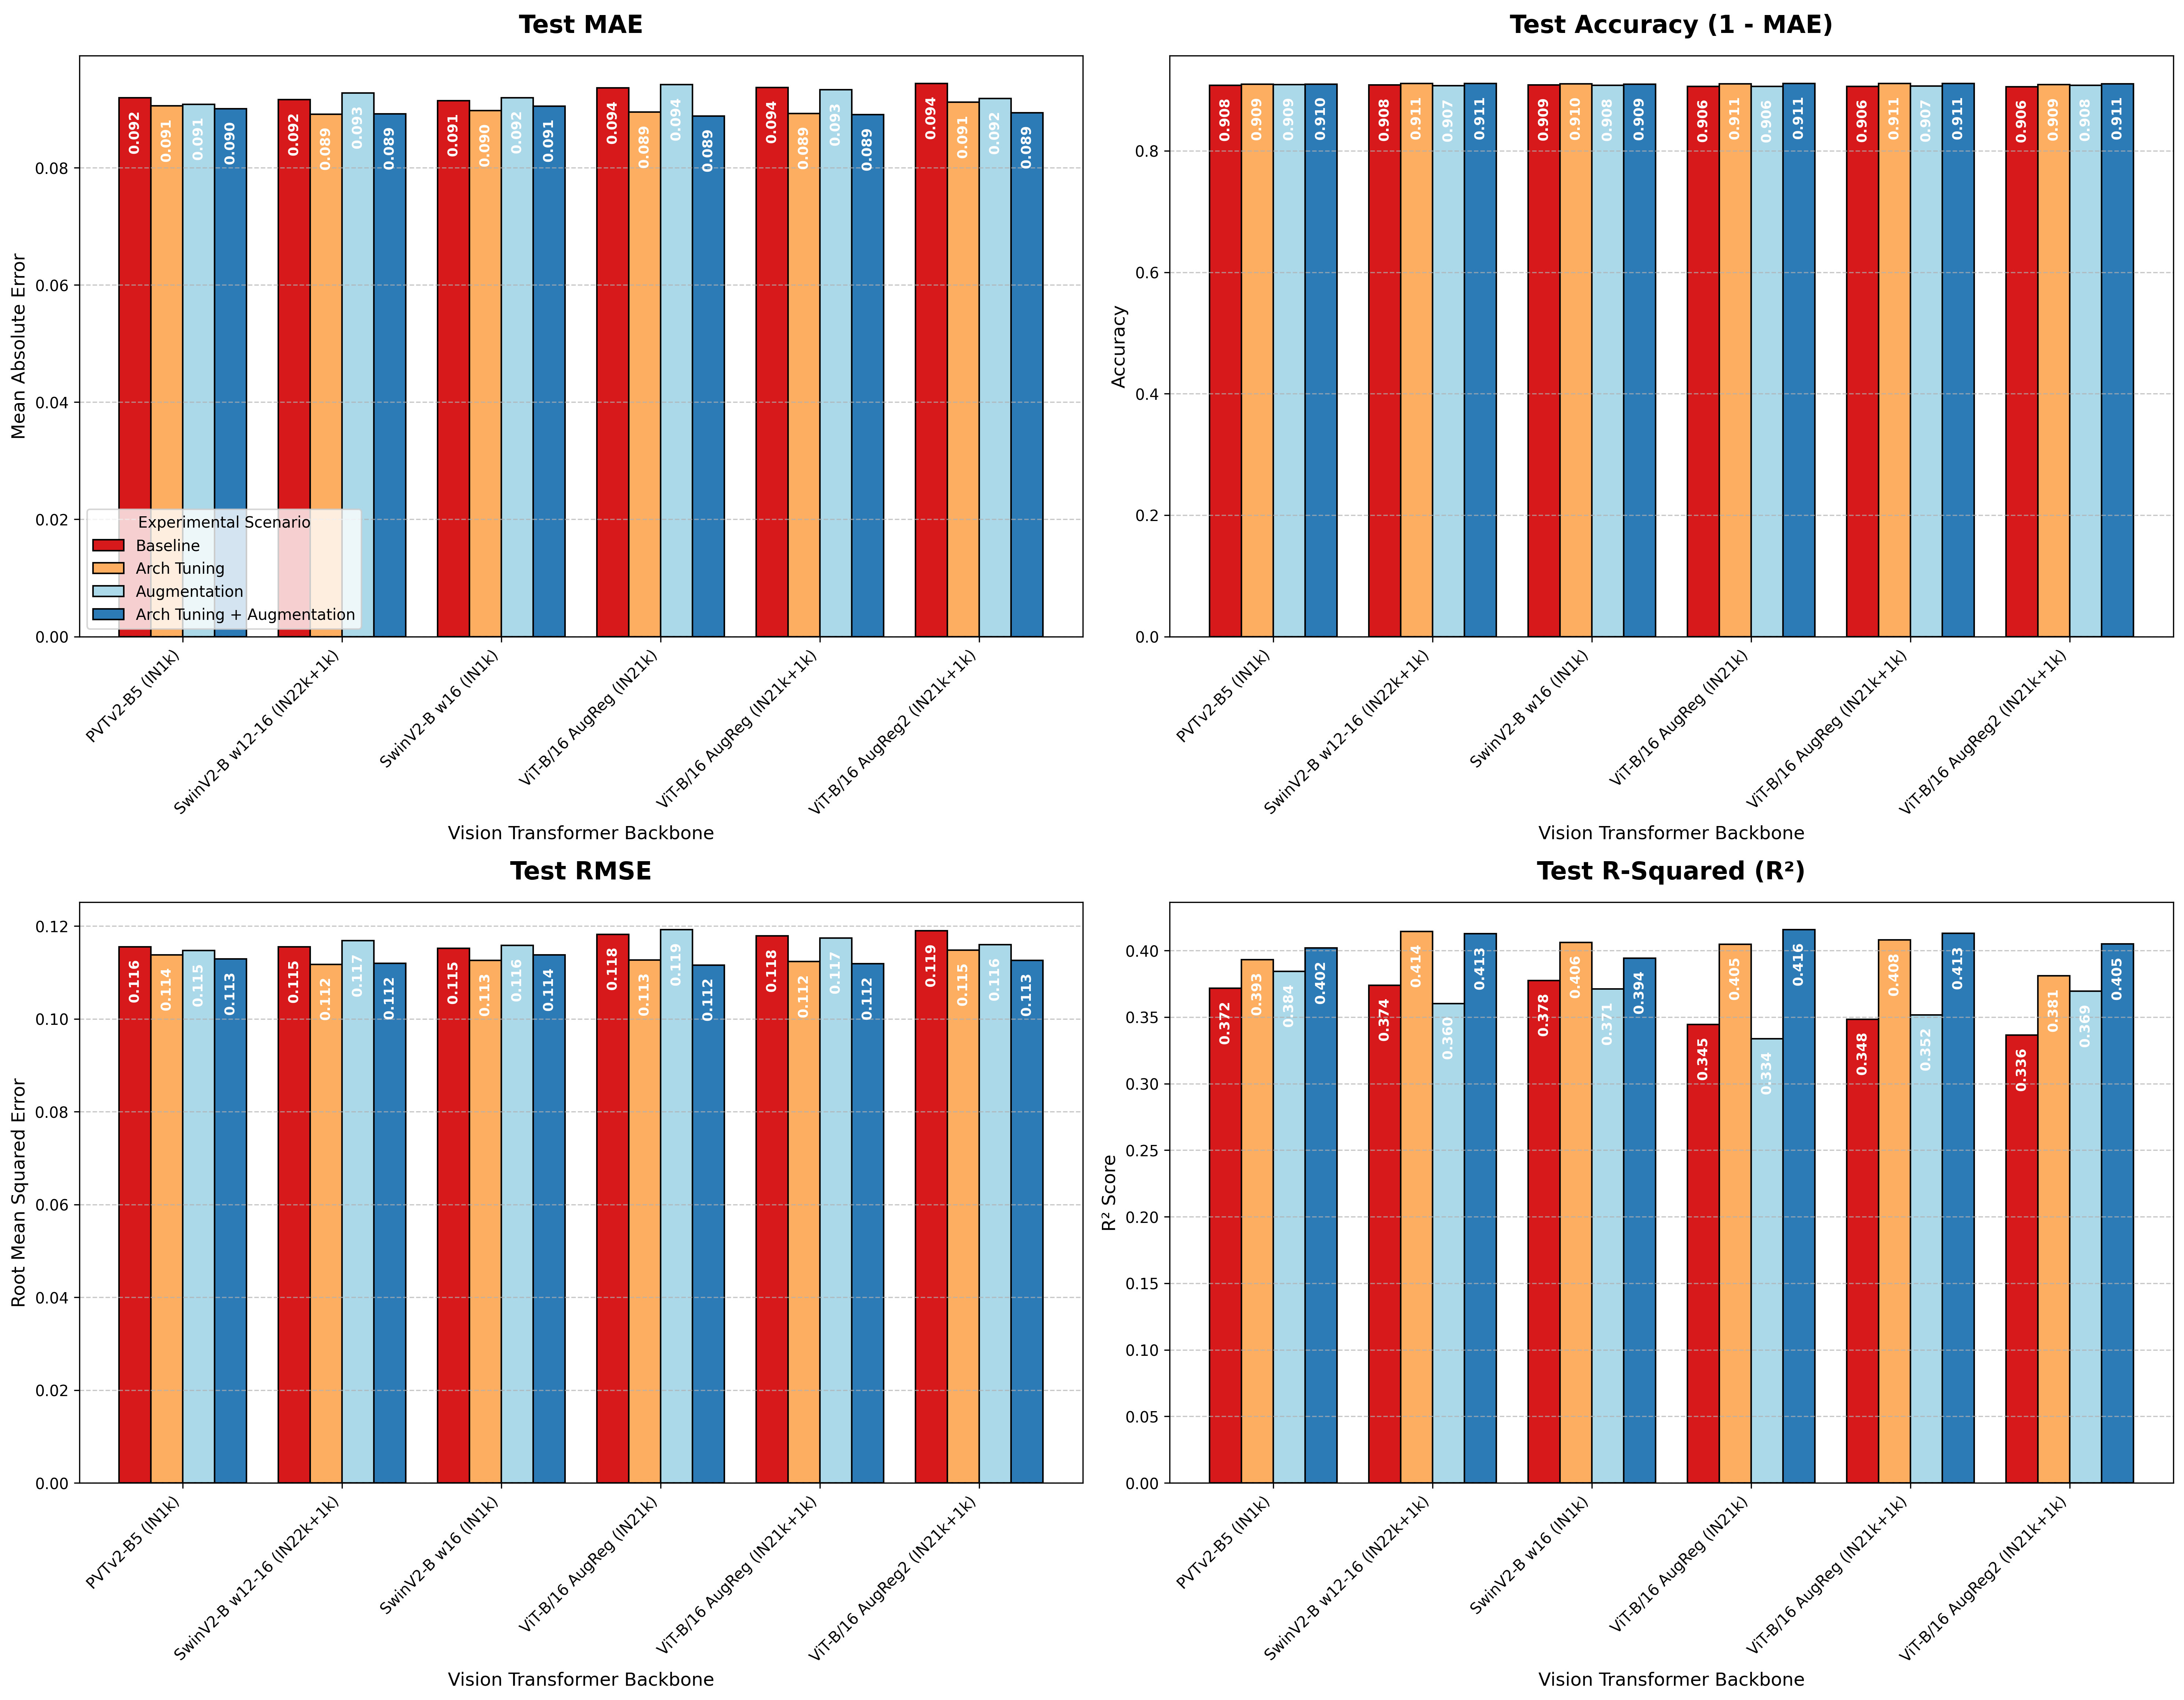
\includegraphics[width=\linewidth]{gambar/pred-model-test-metrics.png}
	\caption{Metrik Kinerja Model pada Dataset \textit{Test}}
	\label{fig:test-set-metrics}	
\end{figure}

Analisis lebih rinci mengenai tingkat presisi model dapat dilihat pada \autoref{tab:accuracy_evaluation} yang menyajikan hasil evaluasi metrik akurasi pada data uji. Nilai numerik yang dicetak tebal pada tabel-tabel evaluasi di subbab ini merepresentasikan pencapaian metrik kinerja terbaik. Berdasarkan tabel tersebut, konfigurasi ViT-B/16 AugReg (IN21k) pada skenario \textit{Arch Tuning + Augmentation} menempati peringkat pertama dengan rata-rata akurasi tertinggi sebesar 0,911. Capaian ini bersaing sangat tipis dengan berbagai konfigurasi lainnya, seperti ViT-B/16 AugReg (IN21k+1k) dan kelompok SwinV2-B w12-16 yang menujukkan kinerja rata-rata akurasi di kisaran 0,910 hingga 0,911. Perbedaan nilai yang kecil ini menunjukkan bahwa sebagian besar arsitektur yang dilengkapi dengan \textit{custom regression head} berhasil mencapai batas kinerja maksimalnya dalam meminimalkan jarak kesalahan absolut secara rata-rata.


{
	\footnotesize 
	\renewcommand{\arraystretch}{1.3} 
	
	\begin{xltabular}{\textwidth}{|
			>{\centering\arraybackslash\hsize=0.3\hsize}X |
			>{\raggedright\arraybackslash\hsize=1.8\hsize}X |
			>{\raggedright\arraybackslash\hsize=1.5\hsize}X |
			>{\centering\arraybackslash\hsize=0.9\hsize}X |
			>{\centering\arraybackslash\hsize=0.9\hsize}X |
			>{\centering\arraybackslash\hsize=0.9\hsize}X |
			>{\centering\arraybackslash\hsize=0.9\hsize}X |
			>{\centering\arraybackslash\hsize=0.9\hsize}X |
			>{\centering\arraybackslash\hsize=0.9\hsize}X |}
		
		% --- 1. CAPTION UTAMA ---
		\caption{Perbandingan Akurasi Model Prediksi Kepribadian pada Berbagai Skenario} 
		\label{tab:accuracy_evaluation} \\
		\hline
		
		% Header Kolom Utama
		\textbf{No} & 
		\textbf{Model} & 
		\textbf{Skenario} & 
		\textbf{\textit{Agree\-able\-ness}} & 
		\textbf{\textit{Con\-sci\-en\-tious\-ness}} & 
		\textbf{\textit{Ex\-traver\-sion}} & 
		\textbf{\textit{Neu\-roti\-cism}} & 
		\textbf{\textit{Open\-ness}} & 
		\textbf{\textit{Average}} \\ \hline
		\endfirsthead
		
		% --- 2. HEADER UNTUK HALAMAN LANJUTAN ---
		\caption*{Lanjutan \autoref{tab:accuracy_evaluation}} \\
		\hline
		\textbf{No} & 
		\textbf{Model} & 
		\textbf{Skenario} & 
		\textbf{\textit{Agree\-able\-ness}} & 
		\textbf{\textit{Con\-sci\-en\-tious\-ness}} & 
		\textbf{\textit{Ex\-traver\-sion}} & 
		\textbf{\textit{Neu\-roti\-cism}} & 
		\textbf{\textit{Open\-ness}} & 
		\textbf{\textit{Average}} \\ \hline
		\endhead
		
		% --- 3. FOOTER HALAMAN ---
		\hline
		\multicolumn{9}{r}{\textit{Berlanjut ke halaman berikutnya...}} \\
		\endfoot
		
		\hline
		\endlastfoot
		
		% --- ISI DATA ---
		1 & ViT-B/16 AugReg (IN21k) & \textit{Arch Tuning} + \textit{Augmentation} & 0,9100 & 0,9169 & 0,9117 & \textbf{0,9072} & \textbf{0,9101} & \textbf{0,9112} \\ \hline
		2 & ViT-B/16 AugReg (IN21k+1k) & \textit{Arch Tuning} + \textit{Augmentation} & 0,9103 & 0,9165 & \textbf{0,9119} & 0,9069 & 0,9091 & 0,9110 \\ \hline
		3 & SwinV2-B w12-16 (IN22k+1k) & \textit{Arch Tuning} & 0,9101 & \textbf{0,9177} & 0,9118 & 0,9057 & 0,9089 & 0,9108 \\ \hline
		4 & SwinV2-B w12-16 (IN22k+1k) & \textit{Arch Tuning} + \textit{Augmentation} & 0,9104 & 0,9170 & 0,9098 & 0,9066 & 0,9100 & 0,9108 \\ \hline
		5 & ViT-B/16 AugReg (IN21k+1k) & \textit{Arch Tuning} & 0,9098 & 0,9171 & 0,9109 & 0,9060 & 0,9097 & 0,9107 \\ \hline
		6 & ViT-B/16 AugReg2 (IN21k+1k) & \textit{Arch Tuning} + \textit{Augmentation} & 0,9099 & 0,9167 & 0,9108 & 0,9066 & 0,9092 & 0,9106 \\ \hline
		7 & ViT-B/16 AugReg (IN21k) & \textit{Arch Tuning} & 0,9104 & 0,9162 & 0,9108 & 0,9060 & 0,9091 & 0,9105 \\ \hline
		8 & SwinV2-B w16 (IN1k) & \textit{Arch Tuning} & \textbf{0,9105} & 0,9166 & 0,9098 & 0,9054 & 0,9090 & 0,9103 \\ \hline
		9 & PVTv2-B5 (IN1k) & \textit{Arch Tuning} + \textit{Augmentation} & 0,9083 & 0,9163 & 0,9102 & 0,9067 & 0,9079 & 0,9099 \\ \hline
		10 & SwinV2-B w16 (IN1k) & \textit{Arch Tuning} + \textit{Augmentation} & 0,9100 & 0,9143 & 0,9091 & 0,9055 & 0,9084 & 0,9095 \\ \hline
		11 & PVTv2-B5 (IN1k) & \textit{Arch Tuning} & 0,9092 & 0,9155 & 0,9093 & 0,9044 & 0,9087 & 0,9094 \\ \hline
		12 & PVTv2-B5 (IN1k) & \textit{Augmentation} & 0,9099 & 0,9142 & 0,9091 & 0,9036 & 0,9091 & 0,9092 \\ \hline
		13 & ViT-B/16 AugReg2 (IN21k+1k) & \textit{Arch Tuning} & 0,9075 & 0,9166 & 0,9087 & 0,9042 & 0,9072 & 0,9088 \\ \hline
		14 & SwinV2-B w16 (IN1k) & \textit{Baseline} & 0,9080 & 0,9135 & 0,9091 & 0,9043 & 0,9078 & 0,9085 \\ \hline
		15 & SwinV2-B w12-16 (IN22k+1k) & \textit{Baseline} & 0,9064 & 0,9143 & 0,9089 & 0,9058 & 0,9067 & 0,9084 \\ \hline
		16 & ViT-B/16 AugReg2 (IN21k+1k) & \textit{Augmentation} & 0,9068 & 0,9126 & 0,9096 & 0,9037 & 0,9081 & 0,9081 \\ \hline
		17 & PVTv2-B5 (IN1k) & \textit{Baseline} & 0,9041 & 0,9158 & 0,9097 & 0,9045 & 0,9062 & 0,9081 \\ \hline
		18 & SwinV2-B w16 (IN1k) & \textit{Augmentation} & 0,9079 & 0,9136 & 0,9081 & 0,9044 & 0,9063 & 0,9080 \\ \hline
		19 & SwinV2-B w12-16 (IN22k+1k) & \textit{Augmentation} & 0,9071 & 0,9136 & 0,9066 & 0,9021 & 0,9069 & 0,9072 \\ \hline
		20 & ViT-B/16 AugReg (IN21k+1k) & \textit{Augmentation} & 0,9039 & 0,9130 & 0,9079 & 0,9041 & 0,9045 & 0,9067 \\ \hline
		21 & ViT-B/16 AugReg (IN21k) & \textit{Baseline} & 0,9051 & 0,9107 & 0,9065 & 0,9035 & 0,9061 & 0,9064 \\ \hline
		22 & ViT-B/16 AugReg (IN21k+1k) & \textit{Baseline} & 0,9060 & 0,9122 & 0,9052 & 0,9036 & 0,9045 & 0,9063 \\ \hline
		23 & ViT-B/16 AugReg (IN21k) & \textit{Augmentation} & 0,9055 & 0,9111 & 0,9073 & 0,9014 & 0,9037 & 0,9058 \\ \hline
		24 & ViT-B/16 AugReg2 (IN21k+1k) & \textit{Baseline} & 0,9038 & 0,9094 & 0,9065 & 0,9013 & 0,9069 & 0,9056 \\ \hline
		\multicolumn{9}{|c|}{} \\[-2ex] \hline
		- & \textit{Blind Random Guess} & - & 0,8533 & 0,8374 & 0,8482 & 0,8524 & 0,8363 & 0,8455 \\ \hline
		
	\end{xltabular}
}

Meskipun metrik akurasi menunjukkan batas kinerja yang hampir seragam, metrik ini belum cukup untuk mendefinisikan kemampuan model dalam menangkap variasi kepribadian secara utuh. Oleh karena itu, penentuan kemampuan generalisasi model juga ditinjau melalui metrik \textit{Test R-Squared} ($R^2$) yang dirangkum pada \autoref{tab:r2_evaluation}. Berbeda dengan fase validasi yang didominasi oleh Swin Transformer, evaluasi $R^2$ pada data uji independen ini menunjukkan arsitektur ViT-B/16 AugReg (IN21k) \textit{Arch Tuning + Augmentation} sebagai model dengan kinerja terbaik. Model tersebut menghasilkan puncak rata-rata $R^2$ sebesar 0,416 dan mengungguli pesaing terdekatnya, yaitu SwinV2-B w12-16 yang berada di angka 0,414. Hasil ini menunjukkan bahwa arsitektur ViT dengan AugReg memiliki ketahanan yang jauh lebih baik terhadap \textit{overfitting} saat dihadapkan pada variasi data baru. Jika digabungkan dengan teknik augmentasi dan \textit{custom regression head}, konfigurasi ini ditetapkan sebagai model inferensi terbaik untuk sistem interpretasi kepribadian.

Analisis lebih mendalam mengenai perbedaan kemampuan prediksi pada masing-masing \textit{trait} kepribadian \textit{Big Five} tidak hanya dapat dilihat dari metrik agregat \autoref{tab:accuracy_evaluation} dan \autoref{tab:r2_evaluation}, tetapi juga divisualisasikan melalui \textit{heatmap} pada \autoref{fig:trait-metrics-heatmap}. Visualisasi \textit{heatmap} ini menggunakan gradasi warna untuk mempertegas perbedaan kinerja prediktif antar \textit{trait}, di mana warna biru tua merepresentasikan tingkat akurasi dan nilai $R^2$ yang tinggi, sedangkan warna kuning merepresentasikan nilai evaluasi yang rendah atau sulit dipelajari secara optimal oleh model. 

%{
%	\footnotesize 
%	\renewcommand{\arraystretch}{1.3} 
%	
%	\begin{xltabular}{\textwidth}{|
%			>{\centering\arraybackslash\hsize=0.3\hsize}X |
%			>{\raggedright\arraybackslash\hsize=1.8\hsize}X |
%			>{\raggedright\arraybackslash\hsize=1.5\hsize}X |
%			>{\centering\arraybackslash\hsize=0.9\hsize}X |
%			>{\centering\arraybackslash\hsize=0.9\hsize}X |
%			>{\centering\arraybackslash\hsize=0.9\hsize}X |
%			>{\centering\arraybackslash\hsize=0.9\hsize}X |
%			>{\centering\arraybackslash\hsize=0.9\hsize}X |
%			>{\centering\arraybackslash\hsize=0.9\hsize}X |}
%		
%		% --- 1. CAPTION UTAMA ---
%		\caption{Perbandingan Nilai $R^2$ Model Prediksi Kepribadian pada Berbagai Skenario} 
%		\label{tab:r2_evaluation} \\
%		\hline
%		
%		% Header Kolom Utama
%		\textbf{No} & 
%		\textbf{Model} & 
%		\textbf{Skenario} & 
%		\textbf{\textit{Agree\-able\-ness}} & 
%		\textbf{\textit{Con\-sci\-en\-tious\-ness}} & 
%		\textbf{\textit{Ex\-traver\-sion}} & 
%		\textbf{\textit{Neu\-roti\-cism}} & 
%		\textbf{\textit{Open\-ness}} & 
%		\textbf{\textit{Average}} \\ \hline
%		\endfirsthead
%		
%		% --- 2. HEADER UNTUK HALAMAN LANJUTAN ---
%		\caption*{Lanjutan \autoref{tab:r2_evaluation}} \\
%		\hline
%		\textbf{No} & 
%		\textbf{Model} & 
%		\textbf{Skenario} & 
%		\textbf{\textit{Agree\-able\-ness}} & 
%		\textbf{\textit{Con\-sci\-en\-tious\-ness}} & 
%		\textbf{\textit{Ex\-traver\-sion}} & 
%		\textbf{\textit{Neu\-roti\-cism}} & 
%		\textbf{\textit{Open\-ness}} & 
%		\textbf{\textit{Average}} \\ \hline
%		\endhead
%		
%		% --- 3. FOOTER HALAMAN ---
%		\hline
%		\multicolumn{9}{r}{\textit{Berlanjut ke halaman berikutnya...}} \\
%		\endfoot
%		
%		\hline
%		\endlastfoot
%		
%		% --- ISI DATA ---
%		\textbf{1} & \textbf{ViT-B/16 AugReg (IN21k)} & \textbf{\textit{Arch Tuning} + \textit{Augmentation}} & \textbf{0,2830} & \textbf{0,5301} & \textbf{0,4534} & \textbf{0,4224} & \textbf{0,3895} & \textbf{0,4157} \\ \hline
%		2 & SwinV2-B w12-16 (IN22k+1k) & \textit{Arch Tuning} & 0,2911 & 0,5348 & 0,4613 & 0,4062 & 0,3784 & \textbf{0,4144} \\ \hline
%		3 & ViT-B/16 AugReg (IN21k+1k) & \textit{Arch Tuning} + \textit{Augmentation} & 0,2864 & 0,5251 & 0,4575 & 0,4163 & 0,3790 & \textbf{0,4129} \\ \hline
%		4 & SwinV2-B w12-16 (IN22k+1k) & \textit{Arch Tuning} + \textit{Augmentation} & 0,2888 & 0,5278 & 0,4381 & 0,4165 & 0,3916 & \textbf{0,4126} \\ \hline
%		5 & ViT-B/16 AugReg (IN21k+1k) & \textit{Arch Tuning} & 0,2790 & 0,5267 & 0,4453 & 0,4070 & 0,3816 & \textbf{0,4079} \\ \hline
%		6 & SwinV2-B w16 (IN1k) & \textit{Arch Tuning} & 0,2933 & 0,5202 & 0,4353 & 0,4019 & 0,3794 & \textbf{0,4060} \\ \hline
%		7 & ViT-B/16 AugReg2 (IN21k+1k) & \textit{Arch Tuning} + \textit{Augmentation} & 0,2739 & 0,5205 & 0,4447 & 0,4097 & 0,3755 & \textbf{0,4049} \\ \hline
%		8 & ViT-B/16 AugReg (IN21k) & \textit{Arch Tuning} & 0,2865 & 0,5190 & 0,4376 & 0,4066 & 0,3736 & \textbf{0,4047} \\ \hline
%		9 & PVTv2-B5 (IN1k) & \textit{Arch Tuning} + \textit{Augmentation} & 0,2702 & 0,5187 & 0,4357 & 0,4208 & 0,3636 & \textbf{0,4018} \\ \hline
%		10 & SwinV2-B w16 (IN1k) & \textit{Arch Tuning} + \textit{Augmentation} & 0,2867 & 0,4971 & 0,4238 & 0,3989 & 0,3647 & \textbf{0,3942} \\ \hline
%		11 & PVTv2-B5 (IN1k) & \textit{Arch Tuning} & 0,2671 & 0,5125 & 0,4260 & 0,3909 & 0,3693 & \textbf{0,3932} \\ \hline
%		12 & PVTv2-B5 (IN1k) & \textit{Augmentation} & 0,2777 & 0,4861 & 0,4187 & 0,3721 & 0,3673 & \textbf{0,3844} \\ \hline
%		13 & ViT-B/16 AugReg2 (IN21k+1k) & \textit{Arch Tuning} & 0,2382 & 0,5250 & 0,4157 & 0,3802 & 0,3460 & \textbf{0,3810} \\ \hline
%		14 & SwinV2-B w16 (IN1k) & \textit{Baseline} & 0,2473 & 0,4840 & 0,4225 & 0,3838 & 0,3501 & \textbf{0,3776} \\ \hline
%		15 & SwinV2-B w12-16 (IN22k+1k) & \textit{Baseline} & 0,2276 & 0,4922 & 0,4162 & 0,3902 & 0,3437 & \textbf{0,3740} \\ \hline
%		16 & PVTv2-B5 (IN1k) & \textit{Baseline} & 0,1944 & 0,5176 & 0,4238 & 0,3871 & 0,3351 & \textbf{0,3716} \\ \hline
%		17 & SwinV2-B w16 (IN1k) & \textit{Augmentation} & 0,2452 & 0,4917 & 0,3989 & 0,3836 & 0,3362 & \textbf{0,3711} \\ \hline
%		18 & ViT-B/16 AugReg2 (IN21k+1k) & \textit{Augmentation} & 0,2311 & 0,4713 & 0,4171 & 0,3701 & 0,3577 & \textbf{0,3695} \\ \hline
%		19 & SwinV2-B w12-16 (IN22k+1k) & \textit{Augmentation} & 0,2269 & 0,4869 & 0,3788 & 0,3610 & 0,3473 & \textbf{0,3602} \\ \hline
%		20 & ViT-B/16 AugReg (IN21k+1k) & \textit{Augmentation} & 0,1877 & 0,4737 & 0,4099 & 0,3786 & 0,3085 & \textbf{0,3517} \\ \hline
%		21 & ViT-B/16 AugReg (IN21k+1k) & \textit{Baseline} & 0,2114 & 0,4714 & 0,3763 & 0,3750 & 0,3075 & \textbf{0,3483} \\ \hline
%		22 & ViT-B/16 AugReg (IN21k) & \textit{Baseline} & 0,1966 & 0,4397 & 0,3871 & 0,3645 & 0,3348 & \textbf{0,3445} \\ \hline
%		23 & ViT-B/16 AugReg2 (IN21k+1k) & \textit{Baseline} & 0,1811 & 0,4376 & 0,3821 & 0,3413 & 0,3400 & \textbf{0,3364} \\ \hline
%		24 & ViT-B/16 AugReg (IN21k) & \textit{Augmentation} & 0,1989 & 0,4483 & 0,3870 & 0,3387 & 0,2963 & \textbf{0,3338} \\ \hline
%		\multicolumn{9}{|c|}{} \\[-2ex] \hline
%		- & \textit{Random Guess} & - & 0,0477 & 0,0528 & 0,0645 & 0,0413 & 0,0464 & \textbf{0,0505} \\ \hline
%		
%	\end{xltabular}
%}


{
	\footnotesize 
	\renewcommand{\arraystretch}{1.3} 
	
	\begin{xltabular}{\textwidth}{|
			>{\centering\arraybackslash\hsize=0.3\hsize}X |
			>{\raggedright\arraybackslash\hsize=1.8\hsize}X |
			>{\raggedright\arraybackslash\hsize=1.5\hsize}X |
			>{\centering\arraybackslash\hsize=0.9\hsize}X |
			>{\centering\arraybackslash\hsize=0.9\hsize}X |
			>{\centering\arraybackslash\hsize=0.9\hsize}X |
			>{\centering\arraybackslash\hsize=0.9\hsize}X |
			>{\centering\arraybackslash\hsize=0.9\hsize}X |
			>{\centering\arraybackslash\hsize=0.9\hsize}X |}
		
		% --- 1. CAPTION UTAMA ---
		\caption{Perbandingan Nilai $R^2$ Model Prediksi Kepribadian pada Berbagai Skenario} 
		\label{tab:r2_evaluation} \\
		\hline
		
		% Header Kolom Utama
		\textbf{No} & 
		\textbf{Model} & 
		\textbf{Skenario} & 
		\textbf{\textit{Agree\-able\-ness}} & 
		\textbf{\textit{Con\-sci\-en\-tious\-ness}} & 
		\textbf{\textit{Ex\-traver\-sion}} & 
		\textbf{\textit{Neu\-roti\-cism}} & 
		\textbf{\textit{Open\-ness}} & 
		\textbf{\textit{Average}} \\ \hline
		\endfirsthead
		
		% --- 2. HEADER UNTUK HALAMAN LANJUTAN ---
		\caption*{Lanjutan \autoref{tab:r2_evaluation}} \\
		\hline
		\textbf{No} & 
		\textbf{Model} & 
		\textbf{Skenario} & 
		\textbf{\textit{Agree\-able\-ness}} & 
		\textbf{\textit{Con\-sci\-en\-tious\-ness}} & 
		\textbf{\textit{Ex\-traver\-sion}} & 
		\textbf{\textit{Neu\-roti\-cism}} & 
		\textbf{\textit{Open\-ness}} & 
		\textbf{\textit{Average}} \\ \hline
		\endhead
		
		% --- 3. FOOTER HALAMAN ---
		\hline
		\multicolumn{9}{r}{\textit{Berlanjut ke halaman berikutnya...}} \\
		\endfoot
		
		\hline
		\endlastfoot
		
		% --- ISI DATA ---
		1 & ViT-B/16 AugReg (IN21k) & \textit{Arch Tuning} + \textit{Augmentation} & 0,2830 & 0,5301 & 0,4534 & \textbf{0,4224} & 0,3895 & \textbf{0,4157} \\ \hline
		2 & SwinV2-B w12-16 (IN22k+1k) & \textit{Arch Tuning} & 0,2911 & \textbf{0,5348} & \textbf{0,4613} & 0,4062 & 0,3784 & 0,4144 \\ \hline
		3 & ViT-B/16 AugReg (IN21k+1k) & \textit{Arch Tuning} + \textit{Augmentation} & 0,2864 & 0,5251 & 0,4575 & 0,4163 & 0,3790 & 0,4129 \\ \hline
		4 & SwinV2-B w12-16 (IN22k+1k) & \textit{Arch Tuning} + \textit{Augmentation} & 0,2888 & 0,5278 & 0,4381 & 0,4165 & \textbf{0,3916} & 0,4126 \\ \hline
		5 & ViT-B/16 AugReg (IN21k+1k) & \textit{Arch Tuning} & 0,2790 & 0,5267 & 0,4453 & 0,4070 & 0,3816 & 0,4079 \\ \hline
		6 & SwinV2-B w16 (IN1k) & \textit{Arch Tuning} & \textbf{0,2933} & 0,5202 & 0,4353 & 0,4019 & 0,3794 & 0,4060 \\ \hline
		7 & ViT-B/16 AugReg2 (IN21k+1k) & \textit{Arch Tuning} + \textit{Augmentation} & 0,2739 & 0,5205 & 0,4447 & 0,4097 & 0,3755 & 0,4049 \\ \hline
		8 & ViT-B/16 AugReg (IN21k) & \textit{Arch Tuning} & 0,2865 & 0,5190 & 0,4376 & 0,4066 & 0,3736 & 0,4047 \\ \hline
		9 & PVTv2-B5 (IN1k) & \textit{Arch Tuning} + \textit{Augmentation} & 0,2702 & 0,5187 & 0,4357 & 0,4208 & 0,3636 & 0,4018 \\ \hline
		10 & SwinV2-B w16 (IN1k) & \textit{Arch Tuning} + \textit{Augmentation} & 0,2867 & 0,4971 & 0,4238 & 0,3989 & 0,3647 & 0,3942 \\ \hline
		11 & PVTv2-B5 (IN1k) & \textit{Arch Tuning} & 0,2671 & 0,5125 & 0,4260 & 0,3909 & 0,3693 & 0,3932 \\ \hline
		12 & PVTv2-B5 (IN1k) & \textit{Augmentation} & 0,2777 & 0,4861 & 0,4187 & 0,3721 & 0,3673 & 0,3844 \\ \hline
		13 & ViT-B/16 AugReg2 (IN21k+1k) & \textit{Arch Tuning} & 0,2382 & 0,5250 & 0,4157 & 0,3802 & 0,3460 & 0,3810 \\ \hline
		14 & SwinV2-B w16 (IN1k) & \textit{Baseline} & 0,2473 & 0,4840 & 0,4225 & 0,3838 & 0,3501 & 0,3776 \\ \hline
		15 & SwinV2-B w12-16 (IN22k+1k) & \textit{Baseline} & 0,2276 & 0,4922 & 0,4162 & 0,3902 & 0,3437 & 0,3740 \\ \hline
		16 & PVTv2-B5 (IN1k) & \textit{Baseline} & 0,1944 & 0,5176 & 0,4238 & 0,3871 & 0,3351 & 0,3716 \\ \hline
		17 & SwinV2-B w16 (IN1k) & \textit{Augmentation} & 0,2452 & 0,4917 & 0,3989 & 0,3836 & 0,3362 & 0,3711 \\ \hline
		18 & ViT-B/16 AugReg2 (IN21k+1k) & \textit{Augmentation} & 0,2311 & 0,4713 & 0,4171 & 0,3701 & 0,3577 & 0,3695 \\ \hline
		19 & SwinV2-B w12-16 (IN22k+1k) & \textit{Augmentation} & 0,2269 & 0,4869 & 0,3788 & 0,3610 & 0,3473 & 0,3602 \\ \hline
		20 & ViT-B/16 AugReg (IN21k+1k) & \textit{Augmentation} & 0,1877 & 0,4737 & 0,4099 & 0,3786 & 0,3085 & 0,3517 \\ \hline
		21 & ViT-B/16 AugReg (IN21k+1k) & \textit{Baseline} & 0,2114 & 0,4714 & 0,3763 & 0,3750 & 0,3075 & 0,3483 \\ \hline
		22 & ViT-B/16 AugReg (IN21k) & \textit{Baseline} & 0,1966 & 0,4397 & 0,3871 & 0,3645 & 0,3348 & 0,3445 \\ \hline
		23 & ViT-B/16 AugReg2 (IN21k+1k) & \textit{Baseline} & 0,1811 & 0,4376 & 0,3821 & 0,3413 & 0,3400 & 0,3364 \\ \hline
		24 & ViT-B/16 AugReg (IN21k) & \textit{Augmentation} & 0,1989 & 0,4483 & 0,3870 & 0,3387 & 0,2963 & 0,3338 \\ \hline
		\multicolumn{9}{|c|}{} \\[-2ex] \hline
		- & \textit{Blind Random Guess} & - & 0,0477 & 0,0528 & 0,0645 & 0,0413 & 0,0464 & 0,0505 \\ \hline
		
	\end{xltabular}
}

% menunjukkan adanya perbedaan kemampuan prediksi pada masing-masing \textit{trait} kepribadian \textit{Big Five}. Berdasarkan kedua metrik tersebut, seluruh model menunjukkan kinerja terbaik dalam memprediksi \textit{trait} \textit{Conscientiousness} dan \textit{Extraversion}. Pada model ViT-B/16, \textit{Conscientiousness} menyentuh tingkat akurasi tertinggi sebesar 0,917 dengan nilai $R^2$ mencapai 0,530 disusul oleh \textit{Extraversion} dengan akurasi 0,912 dan $R^2$ sebesar 0,453. Tingginya kemampuan model dalam memetakan kedua \textit{trait} ini menunjukkan dominasi sifat \textit{Conscientiousness} dan \textit{Extraversion} yang cenderung ditonjolkan melalui fitur fisik yang eksplisit pada gambar, seperti tingkat kerapian penampilan, intensitas senyuman, dan keterbukaan ekspresi wajah.

Berdasarkan visualisasi \textit{heatmap} pada \autoref{fig:trait-metrics-heatmap}, seluruh model secara konsisten menunjukkan kinerja terbaik dalam memprediksi \textit{trait} \textit{Conscientiousness} dan \textit{Extraversion}. Hal ini terlihat jelas dari dominasi warna biru tua pada kedua kolom \textit{trait} tersebut di kedua metrik. Sebagai contoh pada model ViT-B/16, \textit{Conscientiousness} menyentuh tingkat akurasi tertinggi sebesar 0,917 dengan nilai $R^2$ mencapai 0,530, disusul oleh \textit{Extraversion} dengan akurasi 0,912 dan $R^2$ sebesar 0,453. Tingginya kemampuan model dalam memetakan kedua \textit{trait} ini menunjukkan dominasi sifat \textit{Conscientiousness} dan \textit{Extraversion} yang cenderung ditonjolkan melalui fitur fisik yang eksplisit pada gambar diam, seperti tingkat kerapian penampilan, intensitas senyuman, dan keterbukaan ekspresi wajah.

Visualisasi \textit{heatmap} juga dengan sangat kontras menunjukkan karakteristik tantangan setiap \textit{trait} yang diprediksi oleh sistem. Analisis pada \textit{trait} yang paling sulit diprediksi jika ditinjau hanya dari jarak kesalahan absolut menggunakan metrik akurasi, \textit{Neuroticism} menunjukkan nilai paling rendah di angka 0,907. Namun, jika dilihat dari kemampuan model dalam memetakan variasi antar individu yang sebenarnya, \textit{Agreeableness} adalah \textit{trait} yang paling sulit dipelajari oleh seluruh model dengan nilai $R^2$ yang berada di kisaran 0,283 meskipun nilai akurasi tampak aman berada di angka 0,910. Penurunan nilai $R^2$ yang drastis ini menunjukkan batasan modalitas citra statis. \textit{Agreeableness} merupakan \textit{trait} kepribadian yang lebih banyak diekspresikan melalui interaksi sosial yang dinamis atau intonasi suara, sehingga sulit ditangkap secara utuh hanya dari sebuah gambar diam.


\begin{figure}[H]
	\centering
	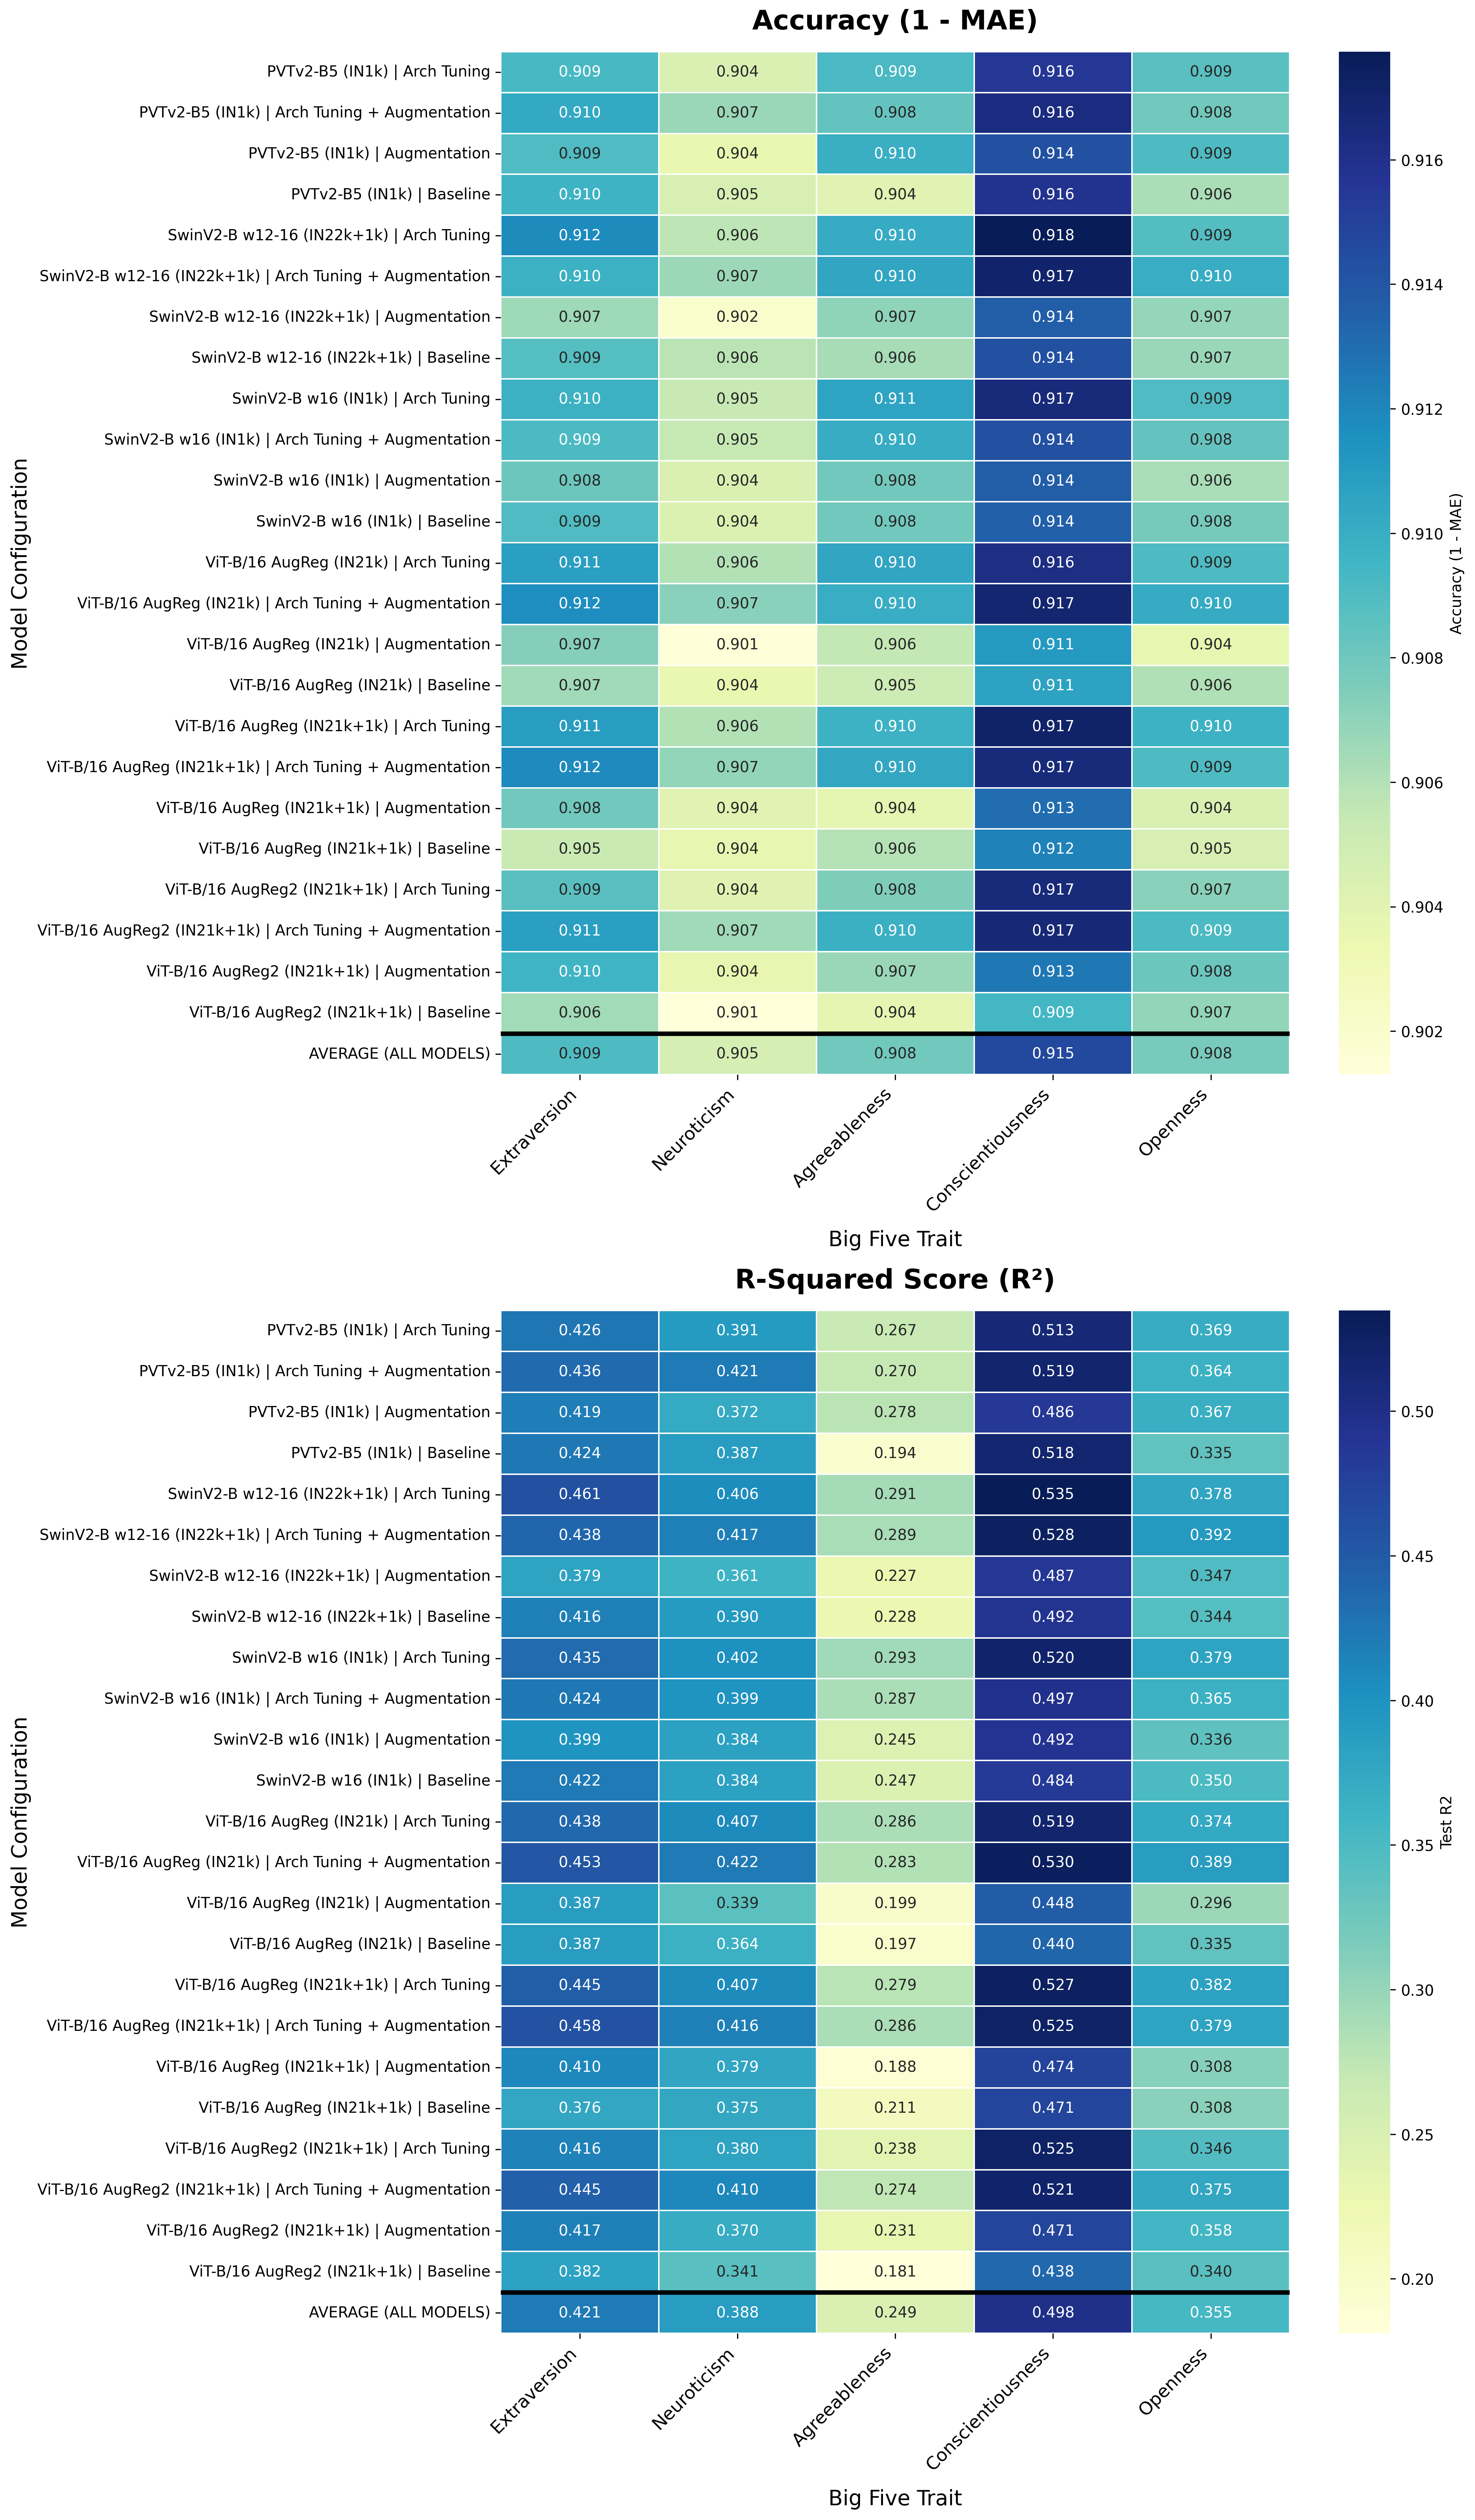
\includegraphics[width=0.85\linewidth]{gambar/trait-metrics-heatmap-grid.png}
	\caption{\textit{Heatmap} Metrik Kinerja Model pada Setiap \textit{Traits}}
	\label{fig:trait-metrics-heatmap}	
\end{figure}

\begin{figure}[H]
	\centering
	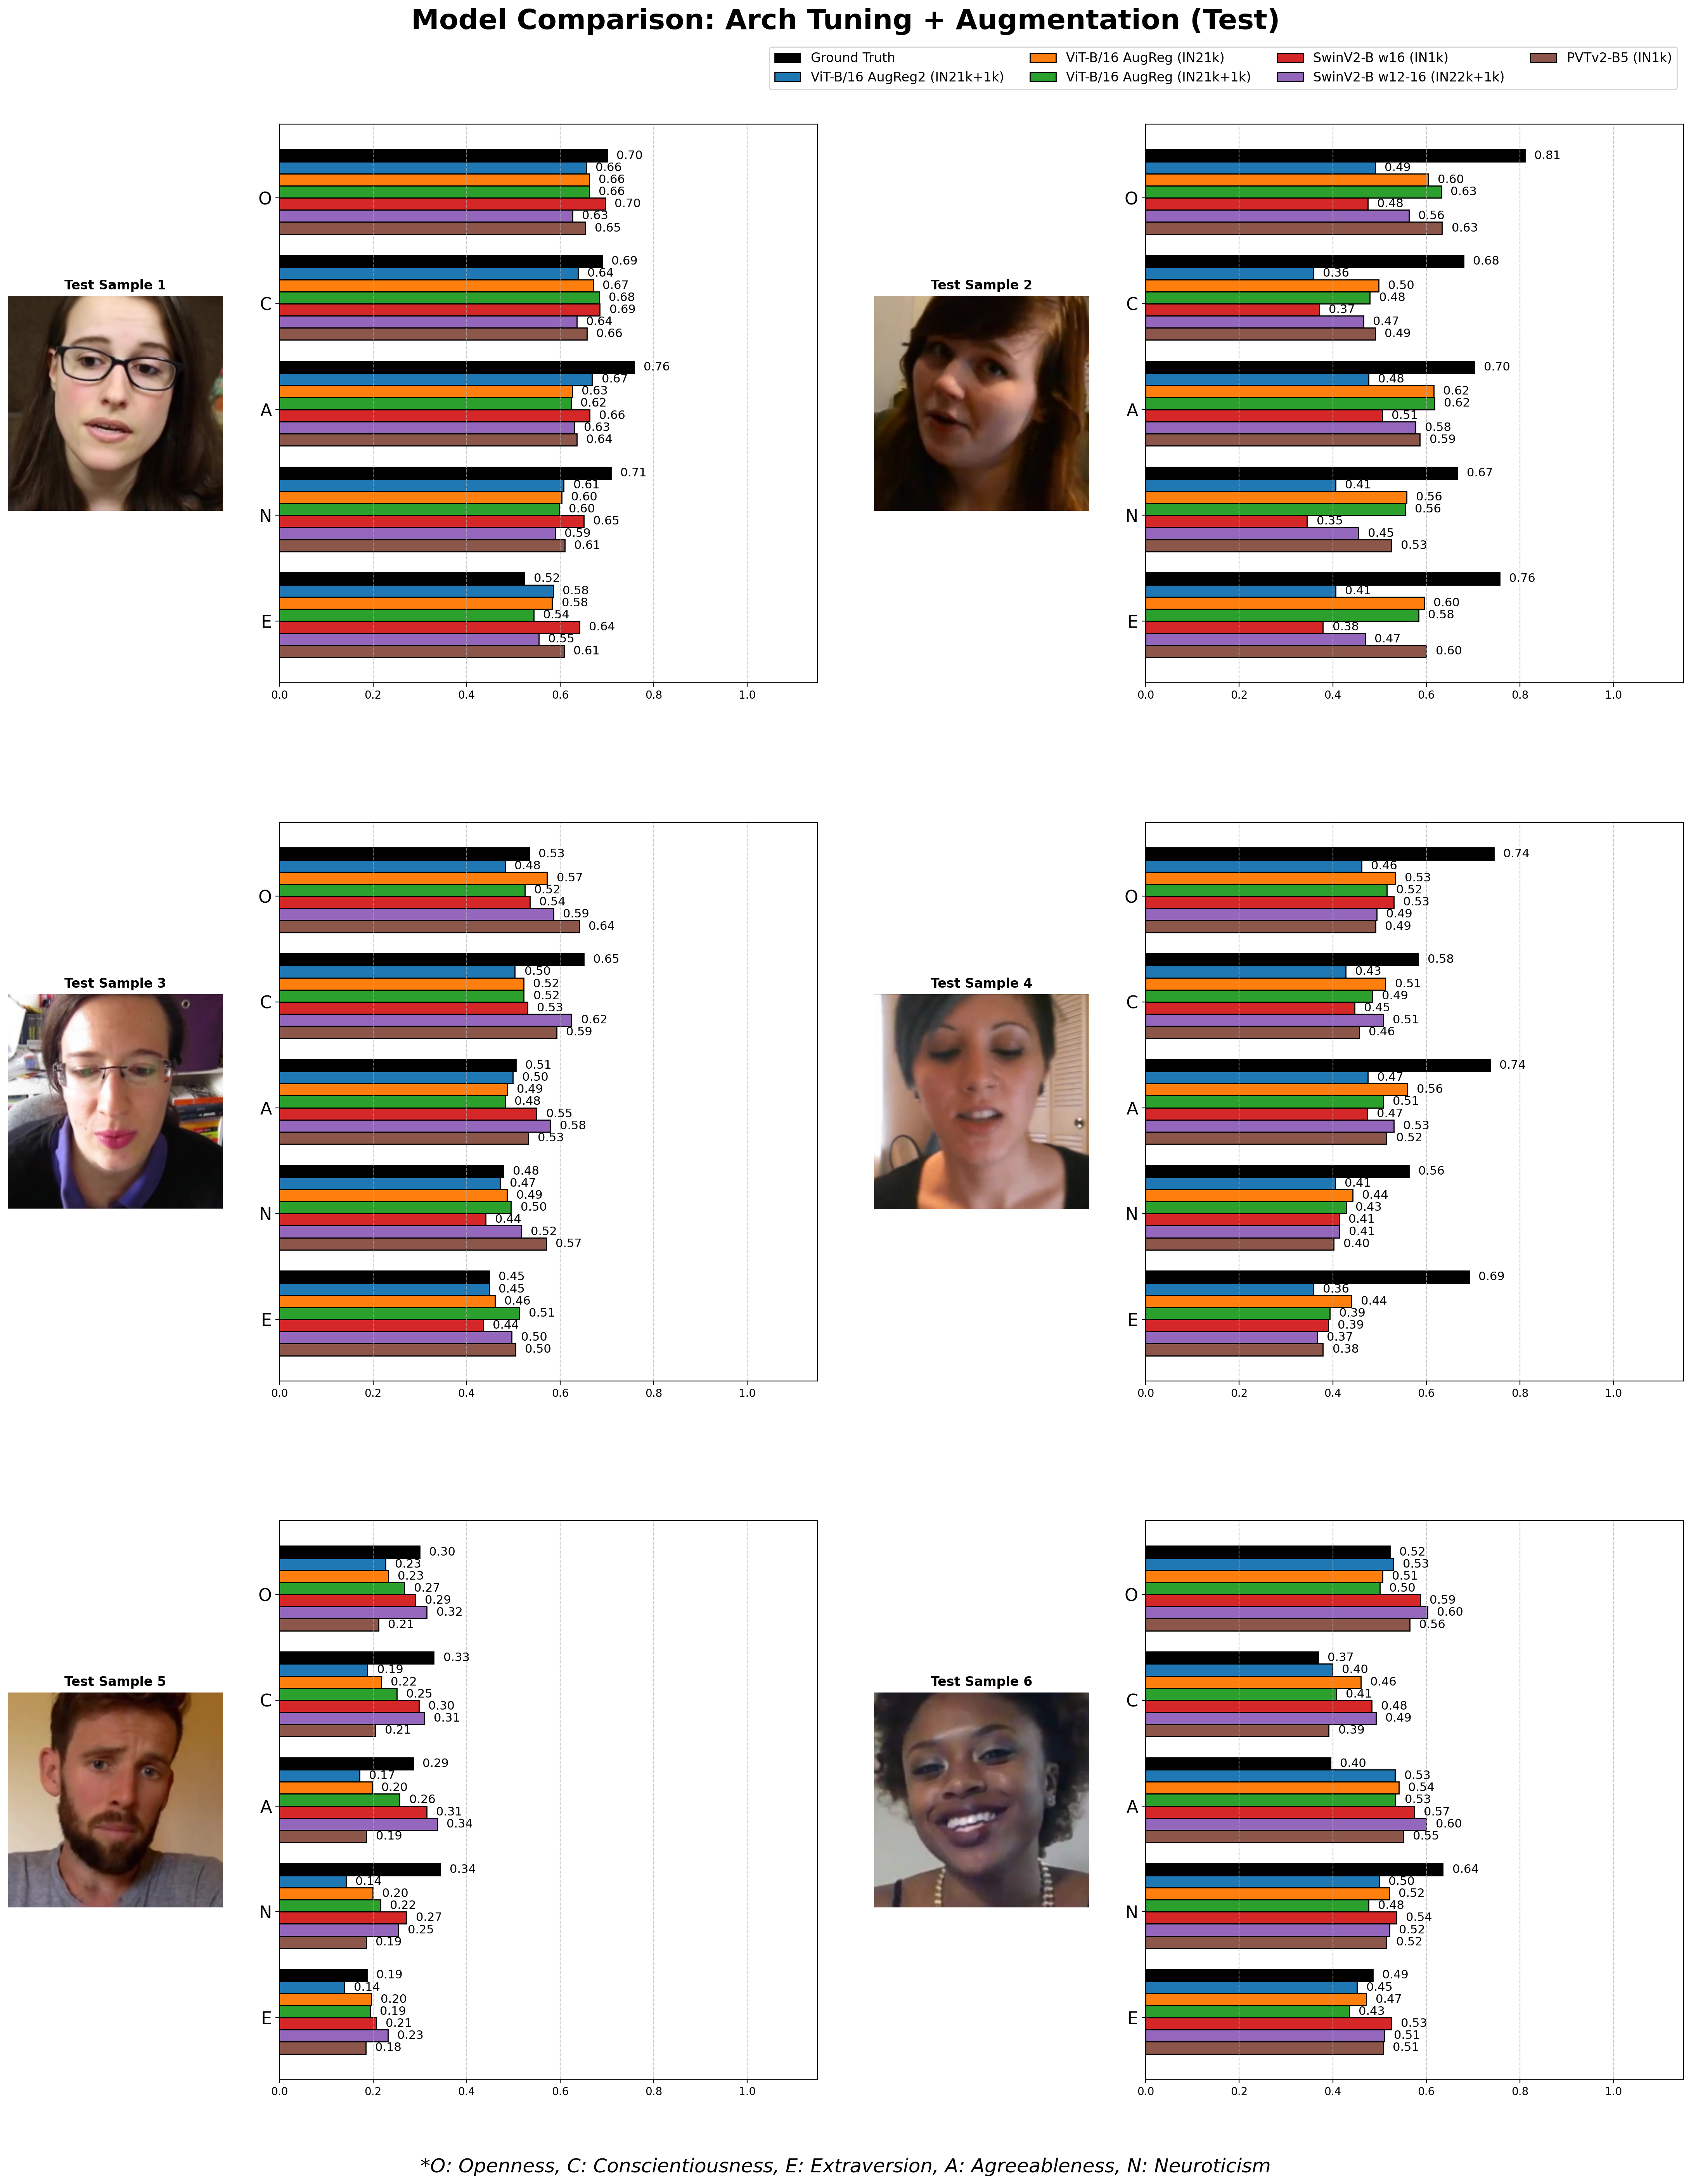
\includegraphics[width=\linewidth]{gambar/all_architectures_Run_D_The_Ultimate_test_showdown.png}
	\caption{Hasil Prediksi Model dengan Skenario \textit{Arch Tuning + Augmentation} pada beberapa Sampel  \textit{Test}}
	\label{fig:sample-prediction-test}	
\end{figure}

Selain melalui metrik agregat, dinamika kinerja model juga dapat dievaluasi dengan melihat sampel prediksi skenario terbaik, yaitu \textit{Arch Tuning + Augmentation} yang divisualisasikan pada \autoref{fig:sample-prediction-test}. Visualisasi ini memperlihatkan fluktuasi nilai prediksi berbagai model saat dihadapkan pada beberapa sampel gambar pengujian. Model pada skenario ini menghasilkan sebaran prediksi yang tidak sekadar menebak skor di sekitar nilai rata-rata populasi tetapi juga menyesuaikan prediksi mengikuti keunikan fitur visual setiap wajah. Namun di sisi lain, visualisasi menunjukkan pada beberapa kasus tertentu, nilai prediksi model masih dapat melenceng cukup jauh dari nilai aktual (\textit{ground truth}). Penyimpangan ini merupakan hasil dari sifat kepribadian manusia yang sangat abstrak. Nilai \textit{ground truth} dalam dataset kepribadian umumnya bergantung pada anotasi pengamat manusia yang cenderung membawa sifat bias kognitif. Selain itu, modalitas citra wajah statis seringkali menampilkan kondisi yang bias seperti sudut pencahayaan, riasan yang menyamarkan fitur asli, atau pose anomali sesaat sehingga tampilan fisik individu pada satu detik tersebut sangat kontras dengan kepribadian aslinya. Adanya kasus-kasus (\textit{outlier}) ini menunjukkan bahwa meskipun sistem prediksi berbasis \textit{computer vision} mampu mengidentifikasi gambaran umum sifat seseorang, kepribadian manusia pada dasarnya terlalu rumit untuk dinilai secara pasti hanya dari sebuah foto statis.

\subsection{Evaluasi Kualitas Interpretasi Kepribadian}

Setelah menetapkan ViT-B/16 AugReg (IN21k) \textit{Arch Tuning + Augmentation} sebagai model regresi terbaik untuk prediksi kepribadian \textit{Big Five}, tahap evaluasi selanjutnya difokuskan pada pengujian kualitas teks hasil interpretasi kepribadian. Tujuan utama dari evaluasi ini adalah untuk mengukur seberapa baik berbagai varian LLM dalam menerjemahkan nilai kepribadian tersebut menjadi narasi profil psikologis yang koheren, akurat, dan empatik berdasarkan gambar dan \textit{prompt} yang diberikan. Pengujian ini mengevaluasi lima varian LLM dari dua keluarga arsitektur utama, yaitu Qwen3-VL (Qwen3-VL-32B-Instruct, Qwen3-VL-235B-A22B-Instruct, dan Qwen3-VL-30B-A3B-Instruct) serta Gemma 4 (Gemma-4-31B-IT dan Gemma-4-26B-A4B-IT). 

Pengujian dilakukan dengan menerapkan dua gaya instruksi utama, yakni \textit{standard prompting} dan \textit{roleplay prompting}. Kedua gaya ini menggunakan basis \textit{prompt} pengguna yang sepenuhnya identik dan memuat input skor prediksi \textit{Big Five} yang didapat dari model prediksi, permintaan analisis fitur visual, serta batasan panjang respons maksimal 1500 token. Perbedaan mendasar hanya terletak pada penambahan \textit{system instruction} pada skenario \textit{roleplay}, di mana model diberikan instruksi untuk mengadopsi persona sebagai seorang psikolog ahli yang sedang memberikan sesi konseling secara empatik dan ramah. Untuk memastikan variasi teks yang sama, seluruh LLM dikonfigurasi dengan nilai \textit{temperature} sebesar 1,0 dan batas maksimal \textit{output} (\textit{max tokens}) ditetapkan pada 2500 token. Evaluasi kualitas teks dilakukan secara menggunakan G-Eval dengan evaluator model GPT-5.1. Untuk memastikan konsistensi dari evaluator \textit{LLM-as-a-judge} tersebut, pengujian dilakukan sebanyak tiga kali iterasi dan nilai akhir ditentukan berdasarkan rata-rata keseluruhan (\textit{grand average}).

Analisis terhadap tiga kriteria penilaian utama (koherensi gambar, akurasi penilaian psikologis, dan persona psikolog) pada \autoref{tab:geval_evaluation_full} menunjukkan ciri khas spesifik dari setiap LLM. Pada metrik akurasi penilaian psikologis, model Gemma 4, terutama varian 26B-A4B pada skenario standar meraih skor tertinggi (0,9566). Hal ini menunjukkan bahwa Gemma 4 sangat presisi dan logis dalam merangkai kalimat agar tidak menyimpang dari skor input \textit{Big Five}. Di sisi lain, keunggulan metrik persona psikolog diraih oleh Qwen3-VL khususnya varian 235B (0,9513), yang menunjukkan kemampuan generatif Qwen dalam merangkai bahasa yang lebih ekspresif dan mendetail. Hal serupa juga terjadi pada metrik koherensi gambar di mana nilai tertinggi dicapai oleh Qwen3-VL-32B pada skenario roleplay dengan skor 0,8740. Jika ditinjau dari rata-rata keseluruhan (\textit{overall average}), Qwen3-VL-32B-Instruct dengan \textit{standard prompting} meraih peringkat tertinggi dengan skor 0,9136. Keberhasilan model dengan parameter 32B dalam mengungguli model yang berukuran jauh lebih besar (235B) menunjukkan bahwa kualitas interpretasi tidak murni ditentukan oleh ukuran parameter, melainkan oleh format bawaan model dalam merespons instruksi tanpa penggunaan persona khusus.

Meskipun beberapa model mencetak rekor di metrik individu, evaluasi ini juga menunjukkan adanya ketimpangan kinerja pada metrik tertentu. Nilai keseluruhan model Gemma-4-26B-A4B-IT jatuh akibat rendahnya kinerja pada metrik koherensi gambar yang hanya berada di angka 0,7929. Hal ini menunjukkan bahwa meskipun varian tersebut sangat bagus merangkai narasi berdasarkan angka, model ini mengalami kesulitan ketika harus mengaitkan analisis teks dengan fitur visual secara natural. Kesenjangan kinerja inilah yang membuat Qwen3-VL-32B menjadi model dengan nilai evaluasi rata-rata terbaik yang mampu menjaga keseimbangan kualitas secara merata di ketiga metrik evaluasi.

Evaluasi ini juga menunjukkan adanya pengaruh \textit{system instruction} yang sangat bergantung pada karakteristik model dasar. Pada model Gemma 4, injeksi persona \textit{roleplay} menunjukkan efektivitas dalam peningkatan skor persona psikolog yang ditunjukkan oleh kenaikan skor Gemma-4-26B-A4B dari 0,9204 menjadi 0,9383. Kenaikan ini menunjukkan bahwa instruksi bertema konseling berhasil mengubah kecenderungan respons model Gemma menjadi narasi yang jauh lebih empatik. Namun fenomena sebaliknya terlihat secara umum, di mana pendekatan \textit{standard prompting} justru cenderung meraih skor rata-rata yang lebih tinggi pada penilaian G-Eval.

Fenomena ini memberikan informasi mengenai cara kerja \textit{LLM-as-a-judge} (G-Eval). Tanpa adanya injeksi persona (\textit{standard prompt}), LLM secara \textit{default} akan menjawab basis instruksi dengan gaya yang analitis dan memecah solusi menjadi poin-poin yang terstruktur. Sistem evaluator G-Eval mengasosiasikan kualitas kepakaran psikolog dengan gaya bahasa laporan klinis yang terstruktur. Format poin per poin yang memisahkan skor dan analisis visual dengan jelas lebih mudah dipindai dan dinilai tinggi oleh G-Eval. Sebaliknya, ketika \textit{roleplay prompt} ditambahkan dalam instruksi interpretasi, teks berubah menjadi lebih natural layaknya sesi dialog antara manusia. Meskipun pendekatan naratif bebas ini terasa lebih bersahabat di mata pengguna manusia, format ini justru dianggap kurang terstruktur oleh G-Eval sehingga menghasilkan skor agregat yang lebih rendah. Perlu menjadi catatan pula bahwa kecenderungan naratif yang bebas pada Qwen3-VL menimbulkan tantangan tersendiri. Model ini sering kali mengabaikan batasan instruksi \textit{prompt} (1500 token) dan menghasilkan respons yang sangat panjang hingga menyentuh \textit{hard limit} sistem (2500 token), yang berisiko memotong respons secara paksa.

Berdasarkan kinerja metrik beserta kelebihan dan kekurangan yang telah dijelaskan, penelitian ini menyimpulkan bahwa tidak ada satu model tunggal yang mendominasi di semua metrik. Oleh karena itu, pengembangan sistem interpretasi kepribadian ini menggunakan dua model alternatif dengan memilih varian paling seimbang dari masing-masing keluarga LLM. Qwen3-VL-32B-Instruct ditetapkan sebagai model utama yang terpilih karena keberhasilannya mencapai skor rata-rata tertinggi secara keseluruhan serta menjaga keseimbangan yang solid pada koherensi gambar dan persona psikolog. Model ini menjadi pilihan ideal untuk skenario yang memprioritaskan kedalaman interaksi. Selain itu, model Gemma-4-31B-IT ditetapkan sebagai model alternatif. Meskipun varian 26B-A4B mencetak skor tertinggi pada metrik akurasi penilaian psikologis (0,9566), model ini memiliki kelemahan pada analisis visual (0,7929) yang membuat skor rata-rata cukup rendah. Oleh karena itu, varian 31B dipilih karena menawarkan keseimbangan kinerja yang jauh lebih baik dan mampu mempertahankan akurasi psikologis yang tinggi (0,9504) sekaligus menjaga koherensi visual di angka yang solid (0,8541). Dengan mempertahankan kedua model terbaik ini, sistem akhir yang diimplementasikan mampu menawarkan fleksibilitas dengan keunggulan Qwen3-VL-32B-Instruct dalam menyajikan narasi interpretasi yang empatik, serta keandalan Gemma-4-31B-IT dalam menyusun teks secara struktural, seimbang, dan presisi.

{
	\footnotesize
	\renewcommand{\arraystretch}{1.3} % Diperbesar sedikit agar teks yang turun ke baris baru tidak terlalu menempel
	
	% Semua kolom sekarang bertipe X dengan bobot proporsional (total = 6.0)
	% Kolom 1 (Model) mendapat porsi paling besar (1.5)
	\begin{xltabular}{\textwidth}{|
			>{\raggedright\arraybackslash\hsize=1.5\hsize}X |
			>{\centering\arraybackslash\hsize=0.8\hsize}X |
			>{\centering\arraybackslash\hsize=0.9\hsize}X |
			>{\centering\arraybackslash\hsize=0.9\hsize}X |
			>{\centering\arraybackslash\hsize=1.0\hsize}X |
			>{\centering\arraybackslash\hsize=0.9\hsize}X |}
		
		% --- 1. CAPTION UTAMA ---
		\caption{Hasil Evaluasi Metrik Interpretasi Kepribadian G-Eval pada Berbagai Skenario} 
		\label{tab:geval_evaluation_full} \\
		\endfirsthead
		
		% --- 2. HEADER UNTUK HALAMAN LANJUTAN ---
		\caption*{Lanjutan \autoref{tab:geval_evaluation_full}} \\
		\hline
		\textbf{\textit{LLM Model}} & \textbf{\textit{Prompt Style}} & \textbf{Koherensi Gambar} & \textbf{Akurasi Penilaian Psikologis} & \textbf{Persona Psikolog} & \textbf{\textit{Overall Average}} \\ \hline
		\endhead
		
		% --- 3. FOOTER HALAMAN ---
		\hline
		\multicolumn{6}{r}{\textit{Berlanjut ke halaman berikutnya...}} \\
		\endfoot
		
		\endlastfoot
		
		
		% ==========================================
		% TABEL A: RUN 1
		% ==========================================
		\hline
		\multicolumn{6}{|l|}{\textbf{(a) \textit{Evaluation Run} 1}} \\ \hline
		\textbf{\textit{LLM Model}} & \textbf{\textit{Prompt Style}} & \textbf{Koherensi Gambar} & \textbf{Akurasi Penilaian Psikologis} & \textbf{Persona Psikolog} & \textbf{\textit{Overall Average}} \\ \hline
		qwen3-vl-32b-instruct & \textit{standard} & \textbf{0,8674} & 0,9367 & 0,9418 & \textbf{0,9153} \\ \hline
		qwen3-vl-235b-a22b-instruct & \textit{standard} & 0,8326 & 0,9398 & \textbf{0,9512} & 0,9079 \\ \hline
		qwen3-vl-32b-instruct & \textit{roleplay} & 0,8671 & 0,9304 & 0,9209 & 0,9061 \\ \hline
		qwen3-vl-235b-a22b-instruct & \textit{roleplay} & 0,8243 & 0,9463 & 0,9470 & 0,9059 \\ \hline
		gemma-4-31b-it & \textit{standard} & 0,8492 & 0,9482 & 0,9194 & 0,9056 \\ \hline
		gemma-4-26b-a4b-it & \textit{standard} & 0,7952 & \textbf{0,9581} & 0,9198 & 0,8910 \\ \hline
		gemma-4-26b-a4b-it & \textit{roleplay} & 0,7763 & 0,9533 & 0,9389 & 0,8895 \\ \hline
		gemma-4-31b-it & \textit{roleplay} & 0,7939 & 0,9414 & 0,9222 & 0,8858 \\ \hline
		qwen3-vl-30b-a3b-instruct & \textit{standard} & 0,8302 & 0,9138 & 0,9088 & 0,8843 \\ \hline
		qwen3-vl-30b-a3b-instruct & \textit{roleplay} & 0,7799 & 0,9041 & 0,7148 & 0,7996 \\ \hline
		
		\multicolumn{6}{c}{} \\[-1ex]
		\multicolumn{6}{c}{} \\[-1ex]
		
		
		% ==========================================
		% TABEL B: RUN 2
		% ==========================================
		\hline
		\multicolumn{6}{|l|}{\textbf{(b) \textit{Evaluation Run} 2}} \\ \hline
		\textbf{\textit{LLM Model}} & \textbf{\textit{Prompt Style}} & \textbf{Koherensi Gambar} & \textbf{Akurasi Penilaian Psikologis} & \textbf{Persona Psikolog} & \textbf{\textit{Overall Average}} \\ \hline
		qwen3-vl-32b-instruct & \textit{standard} & 0,8715 & 0,9375 & 0,9415 & \textbf{0,9168} \\ \hline
		qwen3-vl-32b-instruct & \textit{roleplay} & \textbf{0,8775} & 0,9330 & 0,9224 & 0,9110 \\ \hline
		gemma-4-31b-it & \textit{standard} & 0,8559 & 0,9508 & 0,9188 & 0,9085 \\ \hline
		qwen3-vl-235b-a22b-instruct & \textit{roleplay} & 0,8294 & 0,9461 & 0,9443 & 0,9066 \\ \hline
		gemma-4-26b-a4b-it & \textit{standard} & 0,8111 & \textbf{0,9552} & 0,9198 & 0,8954 \\ \hline
		qwen3-vl-235b-a22b-instruct & \textit{standard} & 0,7788 & 0,9396 & \textbf{0,9512} & 0,8899 \\ \hline
		gemma-4-31b-it & \textit{roleplay} & 0,8045 & 0,9409 & 0,9237 & 0,8897 \\ \hline
		gemma-4-26b-a4b-it & \textit{roleplay} & 0,7741 & 0,9517 & 0,9368 & 0,8875 \\ \hline
		qwen3-vl-30b-a3b-instruct & \textit{standard} & 0,7992 & 0,9215 & 0,9045 & 0,8751 \\ \hline
		qwen3-vl-30b-a3b-instruct & \textit{roleplay} & 0,7846 & 0,8982 & 0,7136 & 0,7988 \\ \hline
		
		\multicolumn{6}{c}{} \\[-1ex]
		\multicolumn{6}{c}{} \\[-1ex]
		
		
		% ==========================================
		% TABEL C: RUN 3
		% ==========================================
		\hline
		\multicolumn{6}{|l|}{\textbf{(c) \textit{Evaluation Run} 3}} \\ \hline
		\textbf{\textit{LLM Model}} & \textbf{\textit{Prompt Style}} & \textbf{Koherensi Gambar} & \textbf{Akurasi Penilaian Psikologis} & \textbf{Persona Psikolog} & \textbf{\textit{Overall Average}} \\ \hline
		qwen3-vl-235b-a22b-instruct & \textit{roleplay} & 0,8542 & 0,9470 & 0,9486 & \textbf{0,9166} \\ \hline
		qwen3-vl-32b-instruct & \textit{roleplay} & \textbf{0,8773} & 0,9346 & 0,9220 & 0,9113 \\ \hline
		qwen3-vl-235b-a22b-instruct & \textit{standard} & 0,8329 & 0,9447 & \textbf{0,9516} & 0,9097 \\ \hline
		gemma-4-31b-it & \textit{standard} & 0,8573 & 0,9521 & 0,9197 & 0,9097 \\ \hline
		qwen3-vl-32b-instruct & \textit{standard} & 0,8461 & 0,9384 & 0,9416 & 0,9087 \\ \hline
		gemma-4-26b-a4b-it & \textit{roleplay} & 0,8053 & 0,9545 & 0,9392 & 0,8997 \\ \hline
		gemma-4-31b-it & \textit{roleplay} & 0,8003 & 0,9445 & 0,9282 & 0,8910 \\ \hline
		gemma-4-26b-a4b-it & \textit{standard} & 0,7724 & \textbf{0,9566} & 0,9216 & 0,8835 \\ \hline
		qwen3-vl-30b-a3b-instruct & \textit{standard} & 0,8089 & 0,9163 & 0,9125 & 0,8792 \\ \hline
		qwen3-vl-30b-a3b-instruct & \textit{roleplay} & 0,7615 & 0,8945 & 0,7136 & 0,7899 \\ \hline
		
		\multicolumn{6}{c}{} \\[-1ex]
		\multicolumn{6}{c}{} \\[-1ex]
		
		
		% ==========================================
		% TABEL D: GRAND AVERAGE
		% ==========================================
		\hline
		\multicolumn{6}{|l|}{\textbf{(d) \textit{Grand Average Across All Runs}}} \\ \hline
		\textbf{\textit{LLM Model}} & \textbf{\textit{Prompt Style}} & \textbf{Koherensi Gambar} & \textbf{Akurasi Penilaian Psikologis} & \textbf{Persona Psikolog} & \textbf{\textit{Overall Average}} \\ \hline
		qwen3-vl-32b-instruct & \textit{standard} & 0,8617 & 0,9375 & 0,9416 & \textbf{0,9136} \\ \hline
		qwen3-vl-235b-a22b-instruct & \textit{roleplay} & 0,8360 & 0,9465 & 0,9466 & 0,9097 \\ \hline
		qwen3-vl-32b-instruct & \textit{roleplay} & \textbf{0,8740} & 0,9327 & 0,9218 & 0,9095 \\ \hline
		gemma-4-31b-it & \textit{standard} & 0,8541 & 0,9504 & 0,9193 & 0,9079 \\ \hline
		qwen3-vl-235b-a22b-instruct & \textit{standard} & 0,8148 & 0,9414 & \textbf{0,9513} & 0,9025 \\ \hline
		gemma-4-26b-a4b-it & \textit{roleplay} & 0,7852 & 0,9532 & 0,9383 & 0,8922 \\ \hline
		gemma-4-26b-a4b-it & \textit{standard} & 0,7929 & \textbf{0,9566} & 0,9204 & 0,8900 \\ \hline
		gemma-4-31b-it & \textit{roleplay} & 0,7996 & 0,9423 & 0,9247 & 0,8888 \\ \hline
		qwen3-vl-30b-a3b-instruct & \textit{standard} & 0,8128 & 0,9172 & 0,9086 & 0,8795 \\ \hline
		qwen3-vl-30b-a3b-instruct & \textit{roleplay} & 0,7753 & 0,8989 & 0,7140 & 0,7961 \\ \hline
		
	\end{xltabular}
}

